\documentclass[a4paper, 11pt, twoside, openright, fleqn]{report}
\usepackage[utf8]{inputenc}
\usepackage[italian]{babel}
\usepackage{microtype}
\usepackage{changepage}
\usepackage{graphicx}
\usepackage{amsmath}
\usepackage{booktabs}
\usepackage{appendix}
\usepackage{tabularx}
\usepackage{caption}
\usepackage{subcaption}
\usepackage{listings}
\usepackage{enumitem}
\usepackage{color}
\usepackage{xcolor}
\usepackage{adjustbox}
\usepackage{titlesec}
\usepackage{titlepic}

\usepackage{lipsum}

\titleformat{\chapter}[hang]{\normalfont\LARGE\bfseries}{\thechapter.}{1ex}{}{}
\titlespacing*{\chapter}{0pt}{0pt}{1.5em}
\titleformat*{\section}{\LARGE\bfseries}
\titleformat*{\subsection}{\Large\bfseries}
\titleformat*{\subsubsection}{\large\bfseries}
\titleformat*{\paragraph}{\large\bfseries}
\titleformat*{\subparagraph}{\large\bfseries}

\renewcommand\labelitemi{$\circ$}
\setlist[itemize]{topsep=4pt,itemsep=0pt,parsep=2pt}
\setlist[enumerate]{topsep=4pt,itemsep=0pt,parsep=2pt}

\newcommand{\llangle}{\langle\!\langle}
\newcommand{\rrangle}{\rangle\!\rangle}
\newcommand{\fromto}[2]{#1\rightarrow #2\!:\ }

\makeatletter
\renewcommand{\paragraph}{%
	\@startsection{paragraph}{4}%
	{\z@}{1ex \@plus 1ex \@minus .2ex}{-1em}%
	{\normalfont\normalsize\bfseries}%
}
\makeatother

% Box con sfondo colorato per protocolli
\newenvironment{colbox}[2]%
{%
	\par\noindent\hspace{10pt}
	\begin{adjustbox}{minipage=[b]{#2},margin=1ex,bgcolor=#1,cfbox=white}
}{%
	\end{adjustbox}\newline%
}

\definecolor{beige}{rgb}{0.96, 0.96, 0.86}
\colorlet{beige}{beige!70}
\colorlet{mygray}{lightgray!15}


\title{Appunti - Sicurezza delle reti}
\author{Martini Michele {\footnotesize et al.}}
\date{A.A. 2019/2020}
\titlepic{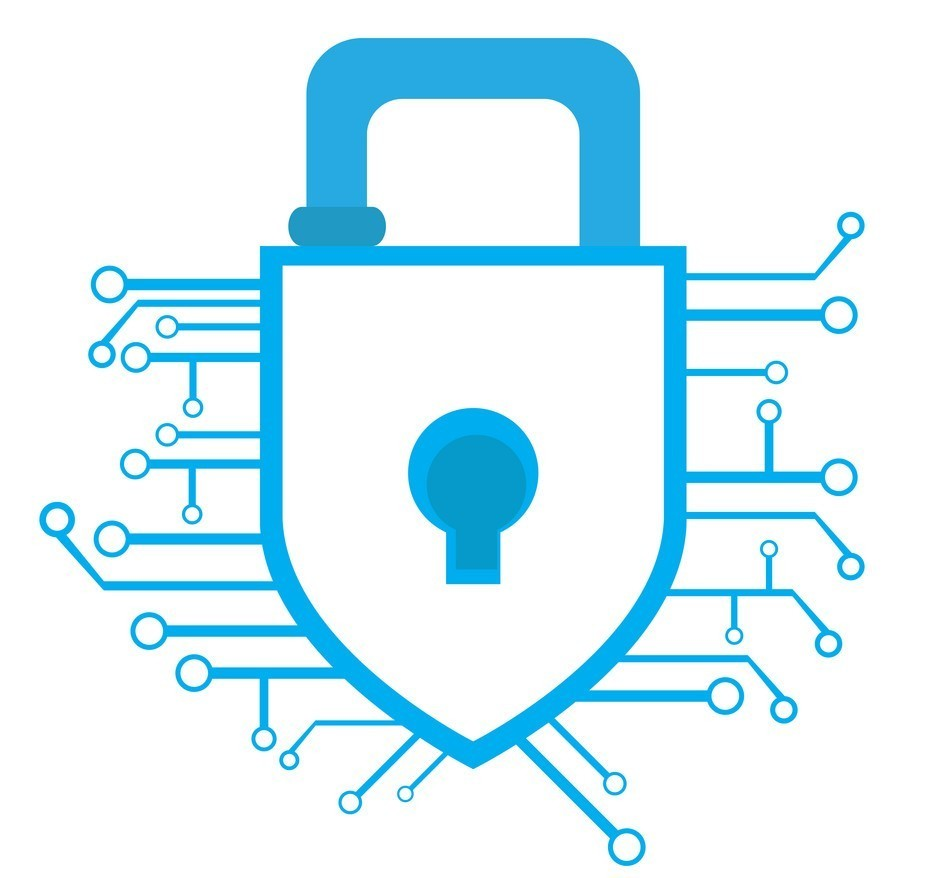
\includegraphics[width=.5\textwidth]{images/logo}}

\begin{document}
\begin{titlepage}
	\begin{adjustwidth}{0cm}{-1.8cm}
	\thispagestyle{empty}
	\centering
	{\huge 
		Appunti\\{\Huge Sicurezza delle reti}\par}
	\vspace{4\baselineskip}
	A.A. 2019/2020\par
	{\textsc{\footnotesize A cura di {\normalsize Michele Martini} et al.}\par}
	\vfil
	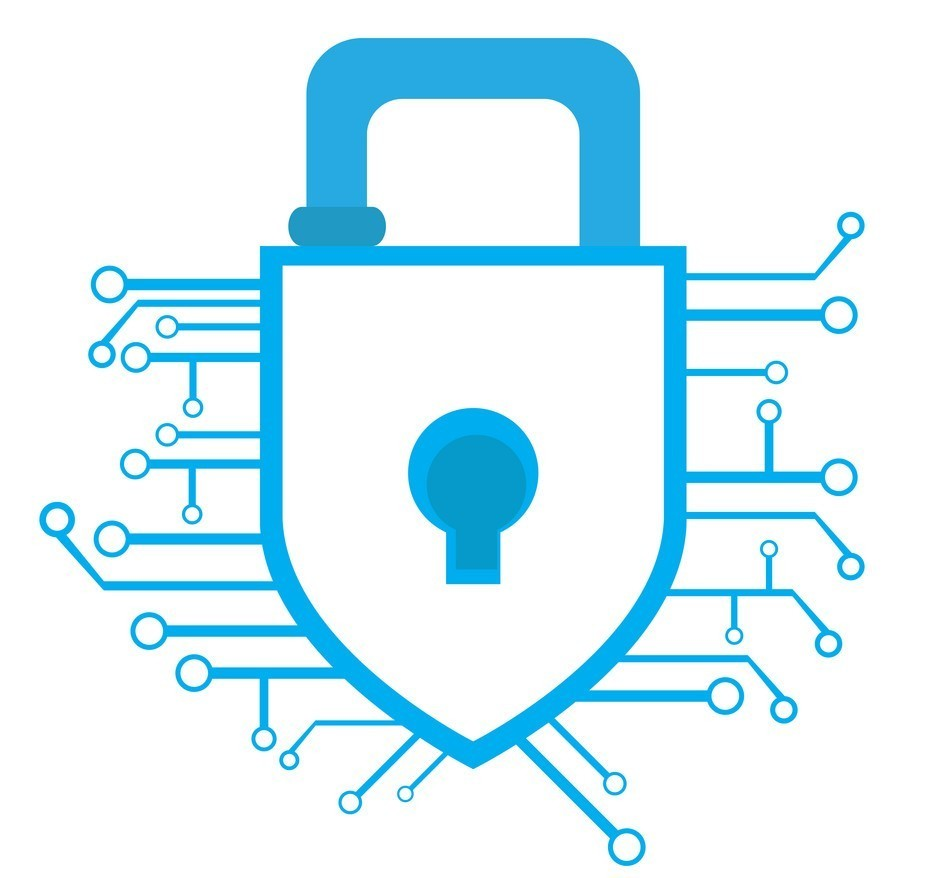
\includegraphics[width=5cm]{images/logo}
		\end{adjustwidth}
\end{titlepage}

\setcounter{tocdepth}{1}
\tableofcontents

\chapter{Sicurezza informatica}
Cosa si intende con \emph{information security}?
\begin{itemize}
	\item \emph{Computer security}\\
	Prevenzione e rilevazione di azioni non autorizzate da parte di utenti di un singolo computer.
	\item \emph{Network security}\\
	Politiche e sistemi adottati dall'amministratore per proteggere la rete e le risorse in essa contenute da accessi non autorizzati.
	\item \emph{Information security}\\
	Sicurezza in senso generico, indica la protezione di informazioni e information systems da accessi/manipolazioni non autorizzati.
\end{itemize}

\section{Sicurezza come policy compliance}
Adottando una prospettiva ben nota in software engineering, possiamo definire i meccanismi di sicurezza per sistemi e risorse in base alla conformità ad una policy o a goals designati:
\begin{itemize}[itemsep=0pt, topsep=6pt]
	\item \emph{Policy:} Specifica dei comportamenti permessi o meno nel sistema.
	\item \emph{Meccanismo:} Meccanismo implementato per imporre la policy.
	\item \emph{Compliance:} Conformità alle specifiche di sicurezza.
\end{itemize}
Al fine di evitare fraintendimenti, diamo una definizione più precisa rigurdo i termini: proprietà, policy e meccanismo.\\
Una \textbf{proprietà} è una descrizione ad alto livello di ciò che si desidera ottenere.\\
Un \textbf{meccanismo} è l'implementazione pratica dei sistemi che permettono l'attuazione di una proprietà.\\
Una \textbf{policy} è la definizione precisa e disambigua di una proprietà, che permette di distinguere un comportamento regolare da uno anomalo. Essa consta di tre parti: prevenzione, detection e risposta.

\subsubsection{Tradizionali proprietà di sicurezza}
Introduciamo e studiamo le più comuni proprietà di sicurezza:
\begin{itemize}[itemsep=0pt]
	\item \emph{Confidentiality}\\
	L'informazione non dev'essere ottenibile/comprensibile da utenti non autorizzati.
	\item \emph{Integrity}\\
	L'informazione non dev'essere modificabile da utenti non autorizzati.
	\item \emph{Availability}\\
	L'informazione dev'essere sempre disponibile.
	\item \emph{Accountability}\\
	Le azioni eseguite devono essere sempre tracciabili.
	\item \emph{Authentication}\\
	I principals e l'origine dei dati devono sempre essere identificabili.
\end{itemize}

\paragraph{Confidenzialità, privacy, segretezza}
Dati e informazioni memorizzate in un sistema o scambiate tra due entità devono essere protette da accessi non autorizzati, ovvero devono risultare accessibili solo agli utenti e ai processi che ne hanno diritto, in base alle policy definite nel sistema. Solitamente se la policy riguarda un singolo individuo parliamo di \emph{privacy}, nel caso di un'organizzazione parliamo invece di \emph{secrecy}. La confidenzialità si ottiene principalmente mediante tecniche crittografiche.\\
NB: privacy $\neq$ anonimity. \emph{Anonimity}: l'identità del principal è celata.

\paragraph{Integrity}
L'integrità garantisce che i dati non vengano alterati da principal malevoli. Essa presuppone una security polity atta ad identificare gli utenti autorizzati alla modifica dei dati (quali utenti possono manipolare quali dati).

\paragraph{Disponibilità}
Questa proprietà assicura l'accesso a dati e servizi in modo affidabile ed in tempi congrui, proteggendo le risorse da: attacchi malevoli, attacchi accidentali (utenti distratti) ed eventi ambientali (es: incendi).\\
Non è sempre facile distinguere un possibile attacco (es: attacco DOS) rispetto ad un uso anomalo ma regolare dei servizi.

\paragraph{Tracciabilità}
La tracciabilità riguarda la registrazione degli eventi per poter risalire ai relativi responsabili. I file in cui vengono salvate le tracce sono detti \emph{secure audit trail/log}. Anche questi file possono essere manipolati se il sistema viene compromesso, perciò vanno trattati adeguatamente (server separato, file di sola lettura, \dots).\\
Una proprietà più stringente della tracciabilità è detta \textbf{non-repudiation}, in cui l'autore di un'azione non può rinnegare di averla compiuta.

\paragraph{Autenticazione}
Dati e servizi devono risultare disponibili solo per utenti autorizzati, in base alle policy definite nel sistema. \`E necessario dunque verificare l'identità di utenti o sistemi, sfruttando uno o più tra i seguenti metodi:
\begin{itemize}
	\item Qualcosa che abbiamo (es: documento)
	\item Qualcosa che conosciamo (es: password)
	\item Qualcosa che siamo (es: impronte digitali)
\end{itemize}


\section{Sicurezza come risk minimization}
La sicurezza informatica si può definire come la protezione delle risorse (dette \emph{asset}) dalle minacce, o \emph{threats}, possiamo dunque decidere di scegliere politiche e meccanismi di sicurezza in base al valore delle risorse ed al rischio di attacco. Questo approccio è ben definito nella pratica, e permette di stabilire con certificati standard la sicurezza del sistema. Valutando le varie minacce, in base alla probabilità di accadimento e all'eventuale impatto sul sistema, possiamo progettare contromisure ad hoc per ciascuna.
\begin{center}
	\texttt{Rischio $=$ Possibilità di accadere $\times$ Impatto sul sistema}
\end{center}
Non possiamo proteggerci da ogni possibile minaccia, in base al fattore di rischio decidiamo se prendere contromisure ed eventualmente quanto investire in quest'ultime.

Quando parliamo in minacce trattiamo sia eventi accidentali sia comportamenti malevoli effettuati da parte di \emph{attaccanti}. Studiamoli dettagliatamente.

\paragraph{Attaccanti}
Gli attaccanti, o \emph{threat agents}, sono utenti che adottano un comportamento malevolo e si possono distinguere in base alle seguenti categorie:
\begin{itemize}
	\item Dipendenti che effettuano azioni dannose involontariamente.
	\item Hacker guidati da sfida personale, usualmente privi di volontà di nuocere.
	\item Ex dipendenti, magari un po' astiosi.
	\item Criminali, terroristi, agenti di spionaggio esteri.
\end{itemize}
Dalla definizione di attaccante ne derivano altre due di pari importanza: \emph{vulnerabilità} e \emph{superficie di attacco}.

\paragraph{Vulnerabilità}
Debolezza del sistema che può essere sfruttata da una minaccia per arrecare un danno.
Le vulnerabilità possono essere dovute all'ambiente fisico (hardware accessibile agli attaccanti), software o di rete. Nel caso una vulnerabilità non sia tuttora nota allo sviluppatore viene detta \emph{zero-day}.

\paragraph{Superficie di attacco}
Parti del sistema esposte a manipolazione da parte di utenti non autorizzati. Tale superficie dev'essere minimizzata per incrementare la sicurezza del sistema. Ad esempio, in ambiente di rete è rischioso lasciare aperte porte non utilizzate dal sistema.\\

\clearpage
\noindent Fasi per l'analisi e la riduzione dei rischi:
\begin{enumerate}
	\item Analisi dei rischi esistenti:
	\begin{itemize}
		\item Identificazione degli asset da proteggere.
		\item Identificazione dei rischi in base a minacce e vulnerabilità.
	\end{itemize}
	\item Analisi delle soluzioni di sicurezza proposte e dei trade-off che ne derivano.
\end{enumerate}


\section{Ingegneria della sicurezza}
\begin{minipage}{0.45\textwidth}
	Far si che il sistema si comporti nei modi specificati $\rightarrow$ \emph{Ingegneria del SW}.
\end{minipage}
\hfill
\begin{minipage}{0.48\textwidth}
	Impedire che il sistema si comporti in modi non specificati $\rightarrow$ \emph{Ingegneria della sicurezza}.
\end{minipage}\\[1em]
Per rendere il sistema sicuro è necessario un approccio \emph{olistico}: la sicurezza deve essere progettata insieme al sistema, non aggiunta successivamente!

L'implementazione di una security solution prevede: analisi e modellazione dei rischi, specifica di security policy, progettazione di adeguate contromisure ed infine studio dei trade-off per decidere quali meccanismi adoperare al fine di rendere sicuro il sistema.\\
Risultano fondamentali i seguenti punti:
\begin{itemize}
	\item Chiarire e documentare gli obiettivi di sicurezza prima dello sviluppo.
	\item Ridurre la complessità mediante tecniche di sviluppo adeguate.
	\item Verificare accuratamente che ogni requisito di sicurezza sia soddisfatto.
\end{itemize}

\section{Metodi formali}
Tecniche e strumenti basati su matematica e logica impiegati nelle fasi di specifica, costruzione ed analisi di sistemi hardware e software. Attraverso i metodi formali è possibile scrivere documentazione non ambigua affinché sia più efficente evitare o almeno individuare errori nell'implementazione. Un modello di sicurezza formale ha il vantaggio di poter distinguere \emph{quali requisiti} il sistema deve poter soddisfare da \emph{come} esattamente esso li soddisfi.


%===============================================================================
\chapter{Meccanismi ed algoritmi crittografici}
Vogliamo trasferire delle informazioni tra due entità: come trasformiamo canali inaffidabili in \emph{canali affidabili}? Prima di tutto dobbiamo definire quali proprietà devono essere soddisfatte dal canale, ad esempio:
\begin{itemize}
	\item Confidenzialità: i dati trasmessi rimangono segreti.
	\item Integrità: le informazioni non sono state alterate.
	\item Autenticazione: i principal conoscono le reciproche idendità.
\end{itemize}
La \emph{tecnologia abilitante} per ottenere tali risultati è la \emph{crittografia}.
\begin{figure}[htp]
	\centering
	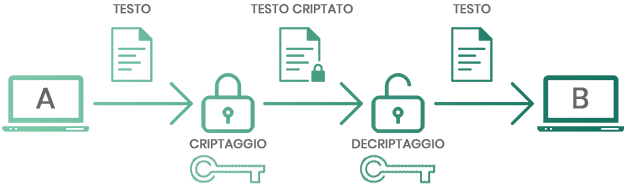
\includegraphics[width=.7\textwidth]{images/Crittografia.png}
	\caption{Schema crittografico generico.}\label{fig:schema-critto}
\end{figure}

\noindent Termini fondamentali:
\begin{itemize}
	\item \emph{Crittologia}: Studio della scrittura segreta.
	\item \emph{Steganografia}: Scienza del nascondere messaggi in altri messaggi.
	\item \emph{Crittografia}: Scienza della scrittura segreta.
	\item \emph{Crittoanalisi}: Scienza del recupero del testo originale da un testo cifrato senza conoscere la chiave di decifratura.
\end{itemize}
In uno schema generico, come in figura [\ref{fig:schema-critto}], abbiamo due agenti A e B che si scambiano un messaggio in chiaro $M$ (anche detto \emph{plaintext} $P$), cifrandolo con una chiave $K_1$ e decifrandolo con una chiave $K_2$, ed indichiamo il testo cifrato con $C$. Distinguiamo principalmente due casi:
\begin{itemize}
	\item Crittografia a chiave simmetrica: $K_1 = K_2$, oppure l'una è facilmente ricavabile conoscendo l'altra.
	\item Crittografia a chiave asimmetrica/pubblica: $K_1 \neq K_2$ e non è possibile usare una delle due chiavi per ricavare l'altra.
\end{itemize}
Se le chiavi sono note, le fasi di cifratura e decifratura dovrebbero essere computazionalmente facili da effettuare.\\
NB: \emph{La sicurezza dipende dalla segretezza della chiave, non dell'algoritmo}.

\begin{figure}[htp]
	\centering
	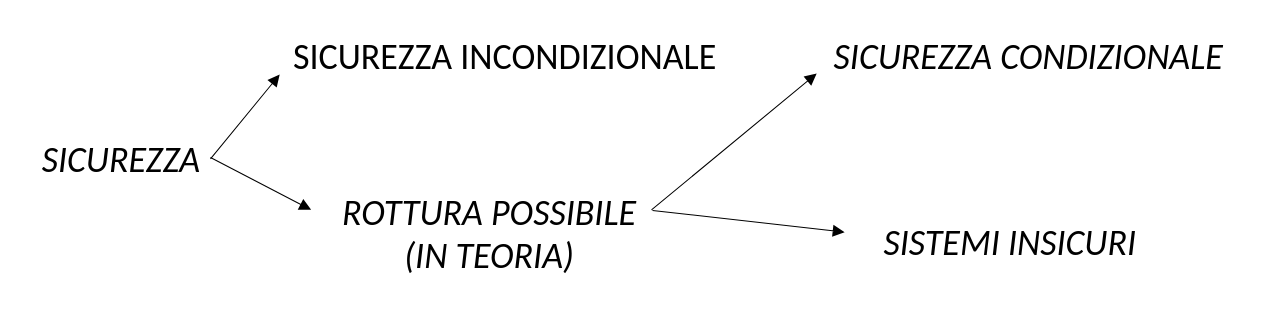
\includegraphics[width=.8\textwidth]{images/Sicurezza_incondizionale.png}
\end{figure}

\paragraph{Unconditional security} Il sistema è sicuro anche se l'avversario disponesse di potenza computazionale illimitata. Si basa sulla \emph{teoria dell'informazione}.\\
\paragraph{Conditional security} Il sistema è teoricamente a rischio, tuttavia per romperlo l'avversario avrebbe bisogno di una potenza computazionale irrealisticamente elevata.

\section{Crittoanalisi}
Obiettivo del crittoanalista è ottenere il testo originale, tuttavia usualmente l'attaccante è interessato anche a recuperare la chiave. Vediamo due approcci comuni:
attacco brute-force e attacco di crittoanalisi.

\paragraph{Brute-force attack}
L'attacco forza-bruta è sempre attuabile e consiste semplicemente nel provare a decifrare il ciphertext con ogni chiave possibile, ammesso di conoscere l'algoritmo e di poter riconoscere il testo originale una volta ottenuto. La complessità cresce esponenzialmente rispetto alla dimensione della chiave.

\paragraph{Attacchi di crittoanalisi}
Da ora in poi assumeremo sempre che l'algoritmo sia noto all'attaccante. Possiamo distinguere vari tipi di attacco in base alle informazioni o ai servizi a cui può accedere l'attaccante:
\begin{itemize}
	\item \emph{Solo testo cifrato}: dati $C_1 = E_K(M_1), \dots, C_n = E_K(M_n)$, l'attaccante può dedurre $M_1, \dots, M_n$ oppure un algoritmo per recuperare $M_{n+1}$ dato $E_K(M_{n+1})$.
	\item \emph{Known plaintext}: dati $M_1, \dots, M_n$ e relativi $C_1, \dots, C_n$, l'attaccante può dedurre la chiave di decifratura oppure un algoritmo per recuperare $M_{n+1}$ dato $E_K(M_{n+1})$.
	\item \emph{Chosen plaintext}: uguale al known plaintext, ma in questo caso l'attaccante può scegliere arbitrariamente i testi in chiaro $M_1, \dots, M_n$.
	\item \emph{Adaptive chosen plaintext}: uguale al chosen plaintext, ma in questo caso l'attaccante può modificare i testi in chiaro da sottoporre a cifratura in base ai risultati delle cifrature precedenti.
	\item \emph{Chosen cyphertext}: L'attaccante può scegliere diversi testi cifrati da decifrare e vederne quindi il testo in chiaro.
\end{itemize}

\clearpage
\subsubsection{Definizione di sicurezza}
Vogliamo garantire una proprietà di sicurezza per il sistema. Per certificare formalmente la soddisfazione dei requisiti di tale proprietà, costruiamo una \emph{definizione di sicurezza} sfruttando il modello in figura [\ref{fig:modello-def-sicurezza}]. Il procedimento prevede le seguenti fasi:
\begin{enumerate}
	\item Specificare un oracolo (ovvero il tipo di attacco).
	\item Definire la condizione di vittoria del gioco per l'attaccante, ovvero una condizione sull'output.
	\item Il sistema è \emph{sicuro} rispetto a quel determinato tipo di attacco se nessun avversario efficente può vincere il gioco con probabilità non trascurabile.
\end{enumerate}
\begin{figure}[htp]
	\centering
	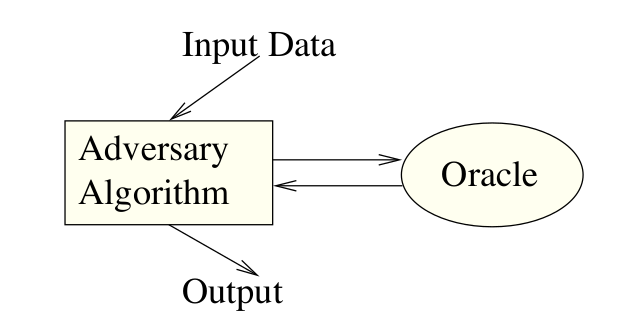
\includegraphics[width=.6\textwidth]{images/Definizione_sicurezza}
	\caption{Modello per costruire una definizione di sicurezza.}\label{fig:modello-def-sicurezza}
\end{figure}

\noindent Esempio di definizione di sicurezza: \emph{conventional encryption}.
\begin{itemize}
	\item Nessun dato in input.
	\item L'avversaro può fare chosen plaintext su un messaggio scelto $M$ o su un testo scelto casualmente.
\end{itemize}
IDEA: Se l'avversario non riesce a distinguere un testo casuale cifrato rispetto al testo cifrato scelto arbitrariamente, non può arrecare alcun danno in casi reali.

\subsubsection{Formalizzazione matematica}
\texttt{Notazione}:
\begin{itemize}
	\item $\mathcal{A}$: l'alfabeto, insieme finito.
	\item $\mathcal{M}\subseteq \mathcal{A}^*$: spazio dei messaggi $\longrightarrow M\in \mathcal{M}$: plaintext.
	\item $\mathcal{C}$: spazio dei messaggi cifrati, il cui alfabeto può essere diverso da $\mathcal{A}$.
	\item $\mathcal{K}$: spazio delle chiavi.
	\item Data $e\in \mathcal{K}$, definiamo $E_e$: funzione di cifratura con chiave $e$ (\emph{encryption function}).
	\item Data $d\in \mathcal{K}$, definamo $D_d$: funzione di decifratura con chiave $d$ (\emph{decryption function}).
\end{itemize}

\paragraph{Schema di cifratura (o cifrario)}
Consiste di un insieme $\{E_e\ |\ e\in K\}$ ed un corrispondente insieme $\{D_d\ |\ d\in K\}$ aventi la seguente proprietà:
\begin{equation*}
	\forall e \in K\,.\,\exists!\;d\in K \quad\mbox{tali per cui}\quad D_d = E_e^{-1}
\end{equation*}
ovvero:
\begin{equation*}
	D_d(E_e(M)) = M, \quad \forall M\in \mathcal{M}
\end{equation*}
Le chiavi $e$ e $d$ formano una \emph{coppia di chiavi} ($e,\,d$).

\section{Cifratura a chiave simmetrica}
Uno schema di cifratura è detto \emph{a chiave simmetrica} se per ogni coppia di chiavi ($e,\,d$) è computazionalmente facile ricavare $d$ da $e$ o viceversa. In pratica: $e=d$. Due principal conoscono una chiave condivisa con cui cifrare/decifrare i messaggi scambiati. Costituiscono tuttora i protocolli crittografici più usati, in quanto risultano molto veloci.\\
Per cifrare messaggi di lunghezza arbitraria vengono usati diversi metodi:
\begin{itemize}
	\item \textbf{Block cipher}: il plaintext viene diviso in blocchi di lunghezza fissa ed ogni blocco viene cifrato separatamente.
	\item \textbf{Stream cipher}: block cipher con lunghezza pari ad 1.
	\item \textbf{Codes}: ad ogni parola è associato un codice identificativo.
\end{itemize}
Studiamo ora diversi tipi di cifratura che sfruttano tecniche di sostituzione, trasposizione o combinazioni di esse.

\subsubsection{Substitution ciphers}
L'idea alla base di questi cifrari consiste nel sostituire ogni lettera del messaggio secondo determinate regole.
\begin{itemize}
	\item \emph{Cifrario di Cesare}: ogni lettera viene "trascinata" di un certo numero di posizioni. La chiave è proprio il numero di posizioni.\\
	\texttt{Debolezza}: brute-force.
	\item \emph{Mono-alfabetico}: generalizzazione del cifrario di Cesare. La chiave è una delle $26!$ permutazioni dell'alfabeto e si associa ad ogni lettera un'altra lettera arbitraria.\\
	\texttt{Debolezza}: analisi delle frequenze.
	\item \emph{Sostituzione omofonica}: sostituisco $a$ con una delle stringhe dell'insieme $H(a)$, in questo modo l'analisi delle frequenze è più difficile ma si complica anche la fase di decifratura.
	\item \emph{Vigenère}: usa la stessa idea del cifrario di Cesare, ma la chiave è composta da più chiavi, es: $K = K_1K_2K_3$. La chiave viene ripetuta sul testo ed ogni lettere del plaintext è cifrata in base alla chiave corrispondente a tale posizione.\\
	\texttt{Debolezza}: analisi delle frequenze con lunghezza della chiave crescente.
	\item \emph{Poli-alfabetico}: usa la stessa idea del cifrario di Vigenère ma ad ogni blocco associa una permutazione diversa invece di uno shift. La chiave è costituita dalla dimensione dei blocchi e dalle permutazioni.
	\item \emph{One-time pad}: il cifrario di Vernam è uno stream cipher con $\mathcal{A}=\{0,1\}$. Effettua uno xor tra plaintext e chiave (di lunghezza pari a quella del messaggio). Il ciphertext non contiene alcuna informazione sul messaggio, ma è difficile per i principals scambiarsi una chiave di tale lunghezza.
\end{itemize}

\subsubsection{Trasposition ciphers}
Le lettere del messaggio originale non vengono sostituite, bensì solo scambiate di posizione. I cifrari basati su trasposizione sono spesso rompibili attraverso analisi delle frequenze.\\[0.5em]
\begin{minipage}{.7\textwidth}
	Classico esempio è la scitala greca: il testo veniva scritto su una cintura ed era comprensibile solo se tale cintura veniva avvolta intorno ad un bastone dell'esatto diametro.
\end{minipage}
\begin{minipage}{.3\textwidth}
	\centering
	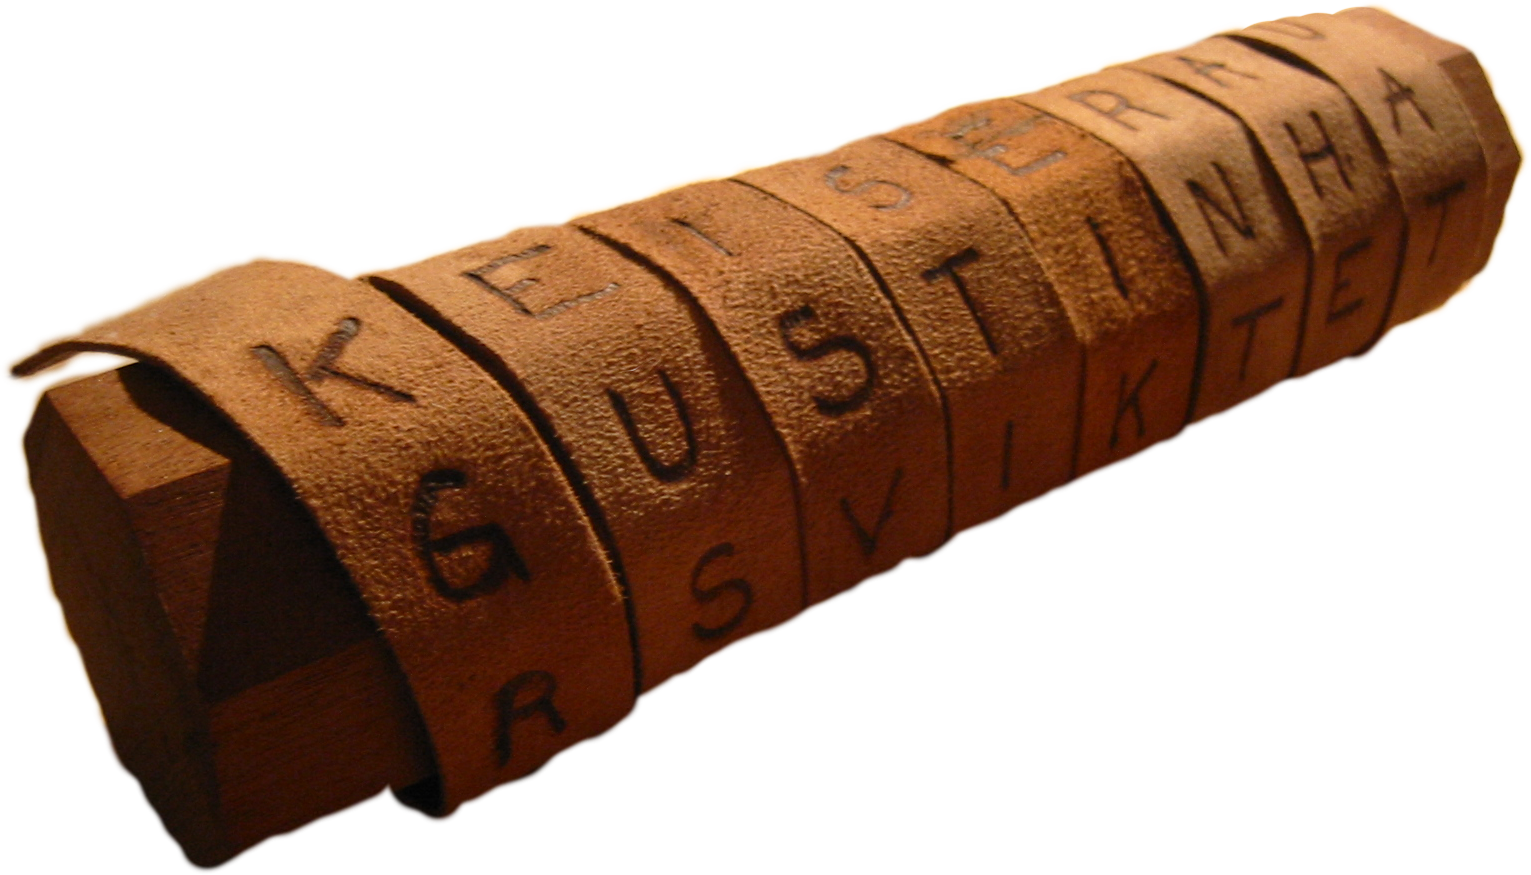
\includegraphics[width=.8\textwidth]{images/Scytale}
\end{minipage}

\subsubsection{Cifrari compositi}
Due sostituzioni poste in cascata sono in realtà una sola sostituzione, così come due trasposizioni in cascata.\\
Sostituzione seguita da trasposizione $\rightarrow$ nuovo cifrario più complesso.
Nel 1949 Shannon introduce le substitution-permutation network:
\begin{itemize}
	\item Substitution $\rightarrow$ confusione del messaggio (nasconde i collegamenti tra plaintext e ciphertext)
	\item Permutation $\rightarrow$ diffonde il messaggio (impedisce l'analisi statistica)
\end{itemize}
\emph{Cifrario di Feistel}: partiziona il plaintext in due metà (HL, HR), esegue $n$ round di cifratura ed infine le concatena nuovamente per formare l'effettivo ciphertext. Ad ogni round:
\begin{enumerate}
	\item applica ad HR una round-function con una chiave;
	\item effettua lo xor con HL;
	\item scambia HL con HR.
\end{enumerate}
\begin{figure}[htp]
	\centering
	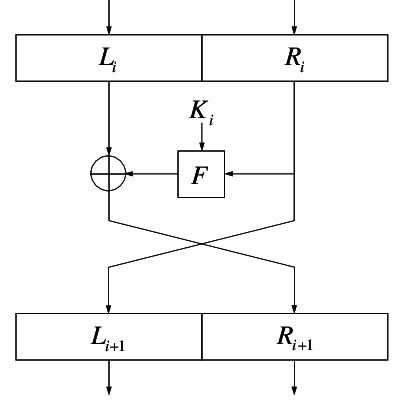
\includegraphics[width=.45\textwidth]{images/Feistel}
	\caption{Round di cifratura di Feistel.}
\end{figure}
\emph{DES}: Data Encryption Standard. Variante di Feistel a 16 round, lavora con chiavi a 56 bit dividendo il testo in blocchi da 64 bit. Possibili atticchi: brute-force o attacco matematico basato su critoanalisi lineare (riduce lo spazio delle chiavi da $2^{56}$ a $2^{43}$).

Vorremmo aumentare la sicurezza di DES per evitare che venga rotto mediante brute-forcing. Se mettiamo due DES in cascata? Double-DES: Non funziona, debole all'attacco \emph{meet-in-the-middle} che riduce lo spazio delle chiavi a $2^{56}$.\\
Triple-DES: tre DES  con due chiavi, $K_1$ e $K_2$, posti in cascata in modo non banale, ovvero:
\begin{itemize}
	\item Encryption: primo e terzo DES cifrano usando $K_1$, mentre il secondo DES decifra con chiave $K_2$.
	\item Decryption: primo e terzo DES decifrano usando $K_1$, mentre il secondo DES cifra con chiave $K_2$.
\end{itemize}
Se $K_1 = K_2$, triplo DES è compatibile con DES. Unico attacco possibile: brute-force con spazio delle chiavi $2^{112}$.

\paragraph{AES:} Advanced Encryption Standard.\\
Evoluzione di triple-DES, in quanto troppo lento e basato su blocchi a 64 bit. AES non ha una struttura di Feistel e lavora con blocchi da 128, 192 o 256 bit.

\paragraph{Plaintext di dimensioni maggiori ad un blocco}
Come può essere applicato un cifrario a blocchi su un messaggio la cui lunghezza eccede le dimensioni del blocco? Esistono molte soluzioni, vediamone solo due:
\begin{itemize}
	\item \emph{Elettronic codebook mode}.\\
	Messaggio spaccato in $m$ blocchi che sono cifrati separatamente.\\
	\texttt{Debolezze}: a blocchi in chiaro uguali corrispondono blocchi cifrati uguali; difficile verificare alterazioni del messaggio cifrato.
	\item \emph{Cipher-block chaining}.\\
	Messaggio spaccato in $m$ blocchi. Prima di cifrare un blocco, viene effettuato lo xor di tale blocco con il testo cifrato di quello precedente:
	\begin{itemize}
		\item[] Encryption: $C_i = E_k(P_i \oplus C_{i-1})$
		\item[] Decryption: $P_i = C_{i-1} \oplus D_k(C_i)$
	\end{itemize}
	La struttura a catena permette il verificarsi di due importanti proprietà:
	\begin{enumerate}
		\item Blocchi uguali sono cifrati in modo diverso.
		\item Se $C_j$ viene alterato ma $C_{j+1}$ no, i blocchi successivi vengono decifrati correttamente.
	\end{enumerate}
\end{itemize}

\section{Posizionamento dell'encryption}
\begin{table}[htp]
\renewcommand{\arraystretch}{1.3}
\begin{tabularx}{\linewidth}{X|X}
	\multicolumn{1}{c}{Link Encryption} & \multicolumn{1}{c}{End-to-End Encryption}\\
	\toprule
	La cifratura è applicata ad ogni link. & La cifratura è applicata solo tra sorgente e destinazione.\\
	Trasparente all'utente. & L'utente deve implementare il protocollo crittografico.\\
	Tutto viene cifrato. & L'utente sceglie cosa cifrare.\\
	Cifratura applicabile anche a livello HW. & Cifratura applicabile solo a livello SW.\\
	Richiede diverse coppie di chiavi. & Chiavi condivise solo tra le due parti della comunicazione.\\
	\emph{Protegge dal monitoring del traffico.} & \emph{Protegge i dati mantenendoli cifrati.}
\end{tabularx}
\end{table}

\section{Crittografia a chiave asimmetrica}
La crittografia a chiave asimmetrica, o a chiave pubblica, viene introdotta come soluzione a due problemi: \emph{distribuzione delle chiavi} e \emph{firma digitale}. Per spiegarne il funzionamento usiamo il classico esempio dell'invio di un messaggio da A a B. 
\begin{enumerate}
	\item A vuole inviare un messaggio $M$ a B.
	\item B crea una coppia di chiavi: ($PU_b,\,PR_b$), $PU_b$ è detta \emph{chiave pubblica}, $PR_b$ è detta \emph{chiave privata}.
	\item A cifra M con la chiave pubblica di B, inviando $C$
	\begin{equation*}
		C=E(PU_b,\,M)
	\end{equation*}
	\item B decifra C usando la propria chiave privata, recuperando $M$
	\begin{equation*}
		M = D(PR_b,\,C) = D(PR_b,\,E(PU_b, M))
	\end{equation*}
\end{enumerate}
\noindent Affinché la crittografia a chiave pubblica sia effettivamente sicura, si rendono necessari alcuni \emph{requisiti}: i passi 2, 3 e 4 devono essere computazionalmente facili da eseguire, mentre dev'essere impraticabile per un avversario:
\begin{itemize}
	\item Determinare $PR_b$ conoscendo $PU_b$.
	\item Determinare $M$ conoscendo $PU_b$ ed esempi di testi cifrati.
\end{itemize}

\begin{table}[htp]
	\renewcommand{\arraystretch}{1.3}
	\begin{tabularx}{\linewidth}{X|X}
		\toprule
		\multicolumn{1}{c|}{\textbf{Simmetric encryption}} & \multicolumn{1}{c}{\textbf{Public-key encryption}}\\
		\toprule
		\multicolumn{2}{c}{\texttt{Requisiti di funzionamento}}\\
		Unici algoritmo e chiave per cifrare e decifrare. & Algoritmi e chiavi diversi per cifrare e decifrare.\\
		I due utenti condividono la chiave e l'algoritmo. & L'utente che invia il messaggio conosce solo la chiave pubblica e l'algoritmo.\\
		\multicolumn{2}{c}{\texttt{Requisiti di sicurezza}}\\
		La chiave deve rimanere segreta. & La chiave privata deve rimanere segreta.\\
		Dev'essere impossibile o impraticabile decifrare un messaggio senza ulteriori informazioni. & Dev'essere impossibile o impraticabile decifrare un messaggio senza ulteriori informazioni.\\
		La conoscenza dell'algoritmo e di testi cifrati dev'essere insufficente a determinare la chiave. & La conoscenza dell'algoritmo, della chiave pubblica e di testi cifrati dev'essere insufficente a determinare la chiave privata.\\
		\bottomrule
	\end{tabularx}
\end{table}

\begin{figure}[htp]
	\centering
	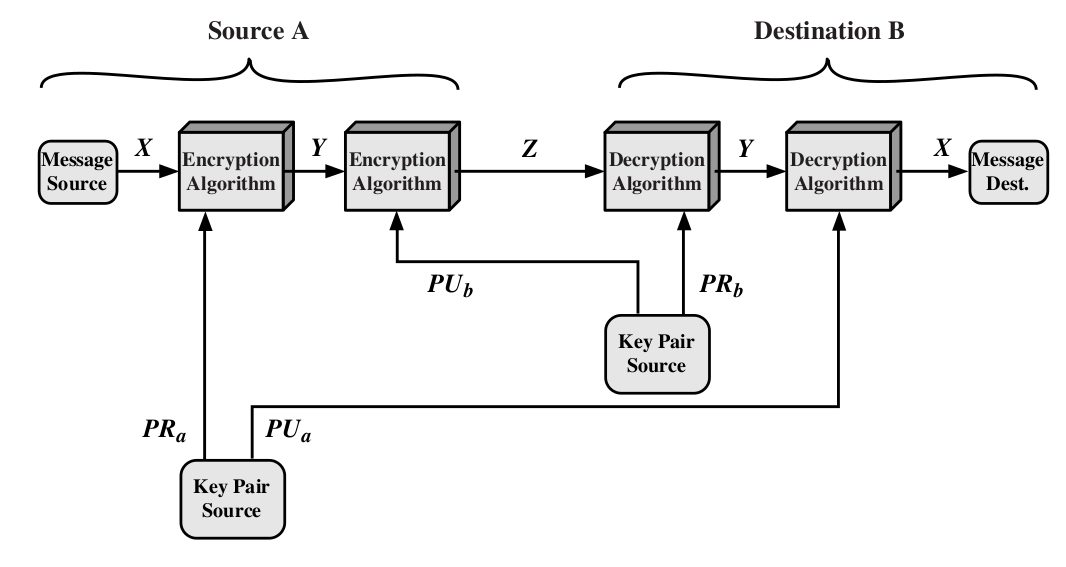
\includegraphics[width=\textwidth]{images/PublicKey}
	\captionsetup{format=hang,width=.8\textwidth}
	\caption{Crittografia a chiave pubblica usata per garantire confidenzialità e autenticazione.}
\end{figure}

\begin{figure}[htp]
	\centering
	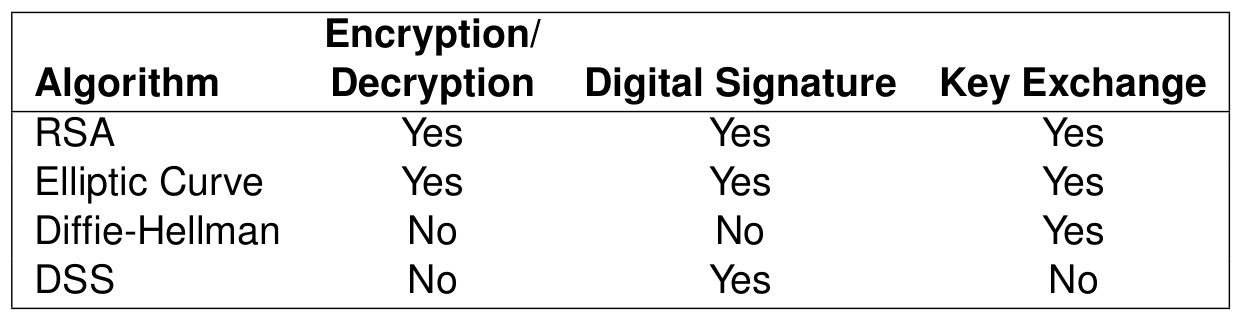
\includegraphics[width=\textwidth]{images/TabellaPK}
	\caption{Soddisfazione dei requisiti di sicurezza dei principali protocolli.}
\end{figure}

\subsubsection{Funzioni one-way trapdoor}
Una funzione $f: X\rightarrow Y$ è detta \emph{one-way} se $f$ è ``facile" da computare $\forall x\in X$, mentre $f^{-1}$ è ``difficile".\\
Una funzione $f_k: X\rightarrow Y$ è detta \emph{one-way trapdoor} se, data l'informazione extra $k$ (\emph{trapdoor information}), è praticabile trovare una $x\in X$ per $y\in Im(f)$ tale che $f_k(x) = y$.

\subsubsection{RSA - Rivest, Shamir, Adleman}
RSA è l'algoritmo crittografico a chiave pubblica più popolare e basa la sua sicurezza sulla difficoltà nel fattorizzare numeri di grandi dimensioni, le chiavi sono infatti numeri primi di oltre 100 cifre. Problema: computazionalmente pesante, per essere sicuro richiede chiavi da 1024 o 2048 bit.

%TODO Aggiungere ref appendice
\clearpage
\paragraph{Funzionamento}
Di seguito sono descritti i passi dell'algoritmo, per comprendere i quali è necessario conoscere alcune basi di teoria dei numeri (vedi appendice).
\begin{itemize}
	\item Generazione delle chiavi:
	\begin{enumerate}
		\item Generiamo 2 numeri primi distinti di almeno 100 cifre: $p$ e $q$.
		\item Computiamo $n=pq$ e $\phi=(p-1)(q-1)$.
		\item Scegliamo $e$ tale che $1<e<\phi$, con $e,\,\phi$ coprimi.
		\item Computiamo $d=e^{-1}\,mod\,\phi$.
		\item Pubblichiamo $PU = (e,\,n)$ e manteniamo segreta $PR = (d,\,n)$.
	\end{enumerate}
	\item Cifratura con chiave $(e,\,n)$:
	\begin{enumerate}
		\item Dividiamo $M$ in $\log_2(n)$ blocchi: $M_1M_2\dots M_l$, con $M_i < n$.
		\item Computiamo $C_i = M_i^e\,mod\,n$.
	\end{enumerate}
	\item Decifratura con chiave $(d,\,n)$:
	\begin{enumerate}
		\item Computiamo $M_i = C_i^d\,mod\,n$.
	\end{enumerate}
\end{itemize}
L'algoritmo funziona in quanto, se la coppia $(e,\,d)$ viene scelta in modo corretto, valgono le seguenti equazioni:
\begin{align*}
	C =& M^e\,mod\,n\\
	M =& C^d\,mod\,n = (M^e)^d\,mod\,n = M^{ed}\,mod\,n
\end{align*}

\paragraph{Sicurezza di RSA}
La sicurezza dell'algoritmo dipende dalla complessità nella risoluzione del problema della fattorizzazione. Non si conoscono algoritmi per risolverlo in tempo polinomiale, tuttavia per rendere impraticabile il calcolo di $d$ dati $e$ ed $n$ è necessario usare chiavi da almeno 1024 bit.

\subsubsection{Problema della distribuzione delle chiavi}
Gli algoritmi a chiave simmetrica sono nettamente più efficenti di quelli a chiave pubblica, tuttavia per funzionare richiedono che mittente e destinatario conoscano la chiave crittografica.
Soluzione: usare un algoritmo a chiave pubblica per scambiarsi una \emph{chiave di sessione}, con la quale cifrare i messaggi scambiati mediante protocolli crittografici simmetrici.\\
Studiamo i seguenti approcci:
\begin{itemize}
	\item RSA
	\item Diffie-Hellman
	\item El Gamal
	\item Massey-Omura
\end{itemize}

\clearpage
\paragraph{Scambio di chiavi con RSA}
\begin{itemize}
	\item Per cifrare $M$ con $PU=(e,\,n)$, scegliamo $k$ casualmente:
	\begin{equation*}
		C = (k^e\,mod\,n,\,E_k(M))
	\end{equation*}
	\item Per decifrare $C$ con $PR=(d,\,n)$, lo dividiamo in $(C_1,\,C_2)$:
	\begin{equation*}
		k = C_1^d\,mod\,n \qquad M=D_k(C_2)
	\end{equation*}
\end{itemize}
I messaggi possono in seguito essere scambiati con crittografia simmetrica con chiave $k$ per una maggior efficenza.\\
Problema: se $d$ viene compromessa in futuro ed un attaccante ha registrato la conversazione, può recuperare i messaggi cifrati.

%TODO Appendice logaritmi discreti
\paragraph{Scambio di chiavi con Diffie-Hellman}
Per poter comprendere il protocollo DH è necessario avere un background riguardo i \emph{logaritmi discreti} (vedi appendice).\\
\texttt{Funzionamento}:
\begin{enumerate}
	\item I principals si scambiano un numero primo $q$ e la \emph{radice primitiva} $\alpha$.
	\item A genera $X_A$ e B genera $X_B$, entrambe inferiori ad $q$.
	\item A genera $Y_A = \alpha^{X_A}\,mod\,q$ e B genera $Y_B = \alpha^{X_B}\,mod\,q$.
	\item A invia $Y_A$ a B mentre B invia $Y_B$ ad A.
	\item A computa $K_A = Y_B^{X_A}$ e B computa $K_B=Y_A^{X_B}$.\\
	Le chiavi $K_A$ e $K_B$ sono uguali:
	\begin{align*}
		K_A &= Y_B^{X_A}\,mod\,q\\
		&= (\alpha^{X_B})^{X_A}\,mod\,q\\
		&= (\alpha^{X_A})^{X_B}\,mod\,q\\
		&= Y_A^{X_B}\,mod\,q = K_B
	\end{align*}
\end{enumerate}
Proprietà di Diffie-Hellman:
\begin{itemize}
	\item[+] Nessuno dei due agenti può sabotare la chiave condivisa generata.
	\item[+] \emph{Perfect Forward Secrecy} (PFS): la chiave di sessione non è compromessa anche se una chiave privata viene scoperta in futuro.
	\item[$-$] Le chiavi non sono autenticate: possibile man-in-the-middle.
\end{itemize}
Man-in-the-middle attack:
\begin{enumerate}
	\item A trasmette $Y_A$ a B.
	\item Z intercetta $Y_A$ e trasmette $Y_Z$ a B.\\
	Inoltre, Z calcola $K_1 = (Y_A)^X_Z\,mod\,q$.
	\item B riceve $Y_Z$ e calcola $K_2 = (Y_Z)^X_B\,mod\,q$.
	\item B trasmette $Y_B$ ad A.
	\item Z intercetta $Y_B$ e trasmette $Y_Z$ ad A.\\
	Inoltre, Z calcola $K_2 = (Y_B)^X_Z\,mod\,q$.
	\item A riceve $Y_Z$ e calcola $K_2 = (Y_Z)^X_A\,mod\,q$.	
\end{enumerate}
A questo punto, A e B credono di condividere una chiave, in realtà A condivide $K_1$ con Z e B condivide $K_2$ con Z.

\paragraph{El Gamal}
Variante di Diffie-Hellman. Partendo dal medesimo setup ($q$ numero primo e $\alpha$ radice primitiva), sfrutta inoltre una funzione crittografica simmetrica $E$:
\begin{enumerate}
	\item B sceglie $X_B$, calcola $Y_B = \alpha^{X_B}\,mod\,q$ e lo invia ad A.
	\item A sceglie $X_A$, calcola $Y_A = \alpha^{X_A}\,mod\,q$, calcola la chiave $K=Y_B^{X_A}\,mod\,q$ ed invia a B questo messaggio: $(E(M,\,K),\,Y_A)$.
	\item B calcola $K=Y_A^{X_B}\,mod\,q$ ed usa $K$ per decifrare $E(M,\,K)$.
\end{enumerate}

\paragraph{Massey-Omura}
Schema di cifratura privo di chiavi condivise, basato sul problema del logaritmo discreto. Il principio per cui funziona è il seguente:
\begin{enumerate}
	\item I principal si scambiano un numero primo $p$ e ognuno dei due sceglie due valori, $e$ e $d$, tali che $ed\,mod\,(p-1) = 1$.
	\item Esiste quindi $k$ tale per cui $ed=k(p-1)+1$.
	\item Per il teorema di Eulero, per ogni $m\in\{1,\,\dots,\,p-1\}$ vale:
	\begin{equation*}
		M^{ed}\,mod\,p = M^{k(p-1)}M\,mod\,p=M\,mod\,p=M
	\end{equation*}
\end{enumerate}

\begin{minipage}{.6\textwidth}
\noindent Funzionamento del protocollo:
\begin{enumerate}
	\item A $\rightarrow$ B: $M^{e_A}\,mod\,p$
	\item B $\rightarrow$ A: $M^{e_Ae_B}\,mod\,p$
	\item A $\rightarrow$ B: $M^{e_Ae_Bd_A}\,mod\,p\ (=M^{e_B})$
	\item B $\rightarrow$ A: $M^{e_Ae_Bd_Ad_B}\,mod\,p\ (= M)$
\end{enumerate}
\end{minipage}
\begin{minipage}{.4\textwidth}
	\centering
	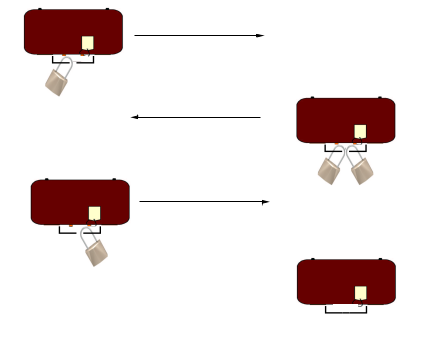
\includegraphics[width=.9\textwidth]{images/MasseyOmura}
\end{minipage}

\subsubsection{Integrità del messaggio}
I dati non possono essere alterati o manipolati da entità non autorizzate, in caso contrario abbiamo gli strumenti per rilevare l'eventuale modifica. Nei sistemi operativi questa proprietà è garantita dal \emph{controllo degli accessi}, in ambito di rete dobbiamo utilizzare la crittografia.\\
IDEA: sfruttare le \emph{funzioni di hash} per creare un'impronta del messaggio. Una funzione di hash $h(x)$ possiede queste proprietà:
\begin{itemize}
	\item \emph{Compressione}: l'output di $h(x)$ è una stringa di lunghezza fissa.
	\item \emph{Efficenza}: $h(x)$ può essere computata in tempo polinomiale.
\end{itemize}
$h(x)$ è una funzione di hash \emph{crittografica} se è inoltre:
\begin{itemize}
	\item \emph{One-way function} (o pre-image resistant).
	\item \emph{2-nd pre-image resistant}: dato $x$, è difficile trovare $x'\ t.c.\ h(x)=h(x')$.
	\item \emph{Collision resistant}: è difficile trovare $x,\,x'\ t.c.\ h(x)=h(x')$.
\end{itemize}
Il valore di hash è detto \emph{message digest} o \emph{modification detection code}.

Un classico impiego delle funzioni hash si ha nei file per lo storing di password, per i quali è sufficiente che la funzione $h$ soddisfi la proprietà di pre-image resistance in quanto combinata con il \emph{sale}.


\subsubsection{Autenticazione del messaggio}
La \emph{message authentication} (detta anche data-origin authentication) comprende l'autenticazione del mittente del messaggio e l'integrità dello stesso. Le principali tecniche per l'autenticazione del messaggio sono \emph{Message Authentication Code} (MAC) e \emph{firma digitale}.

\paragraph{MAC}
Un algoritmo per il Message Authentication Code consiste in una famiglia di funzioni hash $h_k$ parametrizzate da una chiave segreta $k$. Queste funzioni $h_k$ devono essere \emph{computation resistant}: date zero o più coppie di MAC $(x_i,\,h_k(x_i))$, dev'essere impraticabile computare una nuova coppia $(x,\,h_k(x))$ con $x\neq x_i$ senza conoscere la chiave $k$.

Attravarso il MAC possiamo garantire message authentication, ma non la non-repudiation né la freshness. La prima non è verificata in quanto il destinatario B potrebbe creare il messaggio ed applicarvi il MAC fingendo sia stato A ad inviarlo. La \emph{freshness} è una proprietà che indica che il messaggio ricevuto è nuovo, ovvero non è la copia di un vecchio messaggio intercettato da un attaccante e rispedito in seguito (\emph{replay attack}). Il protocollo MAC non garantisce quest'ultima proprietà.

\paragraph{Firma digitale}
La firma digitale (\emph{digital signature}) è un protocollo fondamentale per garantire autenticazione e non-repudiation. Studiamone il funzionamento.
\texttt{Notazione}:
\begin{itemize}
	\item $\mathcal{M}$: spazio dei messaggi.
	\item $\mathcal{S}$: spazio delle firme, ovvero stringhe di lunghezza fissa ($n$-bit).
	\item $S_A\!:\mathcal{M}\rightarrow \mathcal{S}$: creazione della firma per A, tenuta segreta.
	\item $V_A\!: \mathcal{M}\times \mathcal{S}\rightarrow\{true,\,false\}$: verifica pubblica della firma di A.
\end{itemize}
Dati $S_A$ e $V_A$ si può costruire uno schema di firma per A:
\begin{itemize}
	\item \emph{Procedura di firma}\\
	A crea una firma per $M\in\mathcal{M}$, $S=S_A(M)$, e trasmette $(M,\,S)$.
	\item \emph{Procedura di verifica}\\
	B verifica la firma di A, $U=V_A(M,\,S)$, ed accetta il messaggio se e solo se $U=true$.
	\item \emph{Requisiti di sicurezza}\\
	Per chiunque eccetto A dev'essere difficile, dato $M\in\mathcal{M}$, trovare $S\in\mathcal{S}$ tale che $V_A(M,\,S)=true$.
\end{itemize}

\noindent Il meccanismo di firma digitale può essere basato su sistemi crittografici a chiave pubblica \emph{reversibili}, ovvero i sistemi per cui vale $\mathcal{M} = \mathcal{C}$ e vale quindi:
\begin{equation*}
	D_d(E_e(M)) = E_e(D_d(M)) = M\qquad \forall M\in\mathcal{M}
\end{equation*}
Costruiamo lo schema per la firma digitale:
\begin{enumerate}
	\item Siano $\mathcal{M}$ e $\mathcal{C}$ gli spazi di messaggi e firme, $\mathcal{M} = \mathcal{C}$.
	\item Sia $(e,\,d)$ una coppia di chiavi per lo schema di cifratura a chiave pubblica.
	\item Definiamo la funzione di firma $S_A$ per essere $D_d$, ovvero $S=D_d(M)$.
	\item Definiamo $V_A$ come:
	\begin{equation*}
		V_A(M,\,S) =
		\begin{cases}
		true,& \mbox{se }E_e(S) = M\\
		false,& \mbox{altrimenti}
		\end{cases}
	\end{equation*}
\end{enumerate}
Problema: questo schema è vulnerabile ad un \textbf{forgery attack}:
\begin{enumerate}
	\item L'attaccante Z sceglie casualmente una firma $S$ e computa $M=E_e(S)$.
	\item Dato che $\mathcal{C} = \mathcal{M}$, B può inviare $(M,\,S)$ come messaggio firmato.
	\item La verifica ritorna $true$ anche se A non ha firmato il messaggio.
\end{enumerate}
Soluzione:
\begin{itemize}
	\item Nel messaggio viene nominato il mittente.
	\item Firma dell'hash del messaggio al posto dell'intero messaggio.
	\begin{align*}
		\mbox{Firma: } &(M,\,D_d(h(M)))\\
		\mbox{Verifica: } &h(M) = E_e(D_d(M))
	\end{align*}
\end{itemize}
La coppia messaggio-firma può essere cifrata per garantire confidenzialità.

\chapter{Key management}
Quando trattiamo di \emph{key management} ci riferiamo alle infrastrutture che permettono di gestire:
\begin{itemize}
	\item la distribuzione di chiavi crittografiche;
	\item i meccanismi di associazione chiave-identità;
	\item la generazione, il mantenimento e la revoca delle chiavi.
\end{itemize}
Le \emph{Public-Key Infrastructures} (PKI) permettono ai principals di riconoscere i proprietari delle chiavi. Per entrare a far parte della PKI, l'utente A deve:
\begin{enumerate}
	\item Generare una coppia di chiavi, $(PR_A,\,PU_A)$.
	\item Consegnare $PU_A$ ad una \emph{Certification Authority} (CA).
\end{enumerate}
La CA \emph{verifica} l'identità di A e \emph{firma} un certificato che asserisce:
\begin{quote}
	``La chiave $PU_A$ appartiene ad A."
\end{quote}
\begin{minipage}{.62\textwidth}
	\noindent La mutua fiducia nella certification authority permette a due principals di avere un canale sicuro.
\end{minipage}
\begin{minipage}{.38\textwidth}
	\centering
	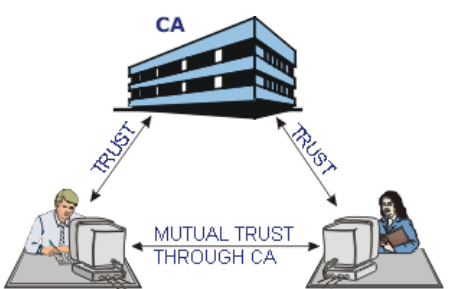
\includegraphics[width=.9\textwidth]{images/CAMutualTrust}
\end{minipage}

\section{Componenti di una PKI}
\begin{figure}[htp]
	\centering
	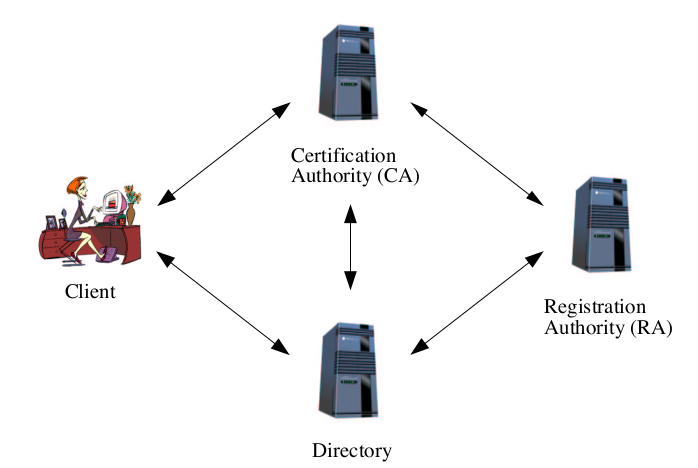
\includegraphics[width=.85\textwidth]{images/PKIComponents}
\end{figure}

\noindent Una PKI può essere \emph{closed} se è limitata ad un gruppo specifico di utenti (es: VPN), oppure \emph{open}. Indipendentemente dal tipo, le componenti di una public-key infrastructure sono: clients, CA, \emph{Registration Authority} (RA) ed una directory.
\begin{itemize}
	\item \emph{Certification Authority}:
	\begin{itemize}
		\item Crea certificati e li pubblica nella directory.
		\item Mantiene la \emph{Certificate Revocation List} (CRL) nella directory.
		\item Esegue il backup di alcune chiavi per recuperi futuri.
	\end{itemize}
	\item \emph{Directory}:
	\begin{itemize}
		\item Server contenente certificati e CRL.
		\item Identifica univocamente gli utenti.
		\item Dev'essere altamente disponibile.
	\end{itemize}
	\item \emph{Registration Authority}:
	\begin{itemize}
		\item Gestisce la registrazione e l'identificazione degli utenti.
		\item Rilascia i nuovi certificati.
	\end{itemize}
	\item \emph{Clients}:
	\begin{itemize}
		\item Autenticazione (one-way, two-way).
		\item Confidenzialità dei messaggi con schema a chiave pubblica.
		\item Firma digitale.
	\end{itemize}
\end{itemize}

\subsection{Certificate revocation and recovery}
Le CRL sono firmate e mantenute dalla CA nella directory, affinché gli utenti possano controllare che un determinato certificato non sia stato revocato. La revoca può scaturire in caso di possibili compromissioni di chiavi private o pubbliche o se l'utente non è più certificato dalla CA.\\
Una CRL contiene:
\begin{itemize}
	\item Nome dell'emittente
	\item Data di creazione della CRL
	\item Data di rilascio della prossima CRL
	\item Una entry per ogni certificato revocato
\end{itemize}
Le CA permettono anche di recuperare le chiavi private, salvandole sui propri server. Ciò può rivelarsi pericoloso, ma è spesso importante averne memorizzata una copia. Mediante \emph{key escrow} una terza parte può recuperare la chiave, spesso per questioni legali.

\subsection{Naming and identity}
Un principal è un'entità univoca, mentre una \emph{identity} è una sua rappresentazione. Compito di una PKI è creare un legame tra un principal e la sua relativa identity. Quest'ultima è difficile da definire, in quanto vogliamo delle policies per l'\emph{assegnamento} e la \emph{risoluzione} dei nomi.\\
X.509 sfrutta i \emph{distinguished names} (DNs) per identificare sia gli utenti che gli emittenti e richiedono la soddisfazione di due criteri:
\begin{itemize}
	\item \emph{Permanenza}: i DNs non devono contenere informazioni volatili.
	\item \emph{Unicità}: i DNs devono essere unici nel tempo.
\end{itemize}
Le CA garantiscono, a certi livelli, per l'identità dei principals a cui viene emesso il certificato:
\begin{itemize}
	\item \emph{CA Authentication policy}\\
	Descrive il livello di autenticazione richiesto per identificare il principal a cui viene emesso il certificato. Stabilisce il livello di dimostrazione di identità richiesto dalla CA per accettare l'affermazione di identità del principal.
	\item \emph{CA issuance policy}\\
	Descrive i principals a cui la CA permette di certificarsi.\\
	(Data l'identità del soggetto, è idoneo alla certificazione?)
\end{itemize}


\section{Certificati}
Un certificato è un \emph{token} che collega un'identità ad una chiave e deve essere firmato da una CA. Il certificato $C_A$ contiene la chiave pubblica dell'utente A, una rappresentazione della sua identità ed un timestamp $T$:
\begin{equation*}
	C_A = M || E(PR_{CA},\,H(M))\qquad \mbox{dove } M=\langle PU_A,\,A,\,T\rangle
\end{equation*}
Come modello di certificato studiamo lo standard \emph{X.509}, su cui si basano struttura e protocolli di autenticazione usati in vari contesti (es: IPSEC, SSL/TLS, \dots). Tale standard si basa su crittografia a chiave pubblica (raccomandato RSA), funzioni hash e firma digitale.

\subsection{Modello X.509}
\begin{minipage}[c]{.52\textwidth}
	Componenti del certificato:
	\begin{itemize}
		\item \emph{Versione del certificato}
		\item \emph{Numero seriale}\\
		La coppia \emph{emittente - numero seriale} identifica univocamente il certificato.
		\item \emph{Signature algorithm identifier}\\
		Algoritmo usato per firmare il certificato.
		\item \emph{Issuer name}\\
		Identificativo della CA.
		\item \emph{Periodo di validità}
		\item \emph{Nome del soggetto}
		\item \emph{Informazioni sulla chiave pubblica}\\
		Algoritmo, parametri e chiave del soggetto.
		\item \emph{Firma}\\
		Contiene l'hash degli altri campi, firmato dalla CA.
	\end{itemize}
\end{minipage}
\hfil
\begin{minipage}{.45\textwidth}
	\centering
	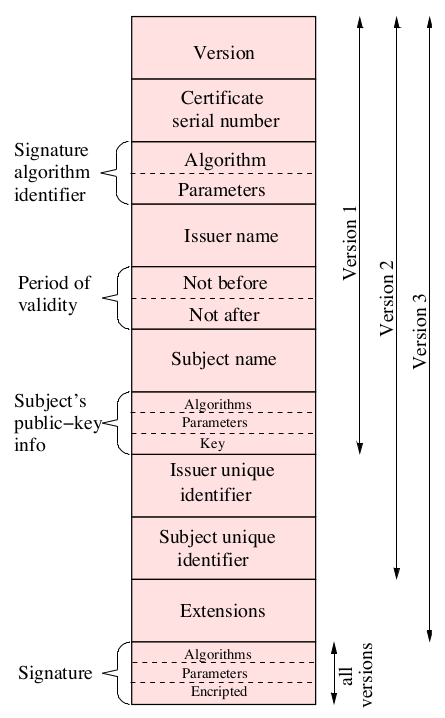
\includegraphics[width=.95\textwidth]{images/X509}
\end{minipage}
\vspace{2em}

\noindent
Certificato di A firmato dalla CA:
\begin{equation*}
	CA\llangle A\rrangle = M \,||\, E(PR_{CA},\,H(M)),\quad
	\mbox{con } M = \langle V,\,SN,\,AI,\,CA,\,T_A,\,A,\,Ap\rangle
\end{equation*}
%dove $M = \langle V,\,SN,\,AI,\,CA,\,T_A,\,A,\,Ap\rangle$.

Chi intende comunicare con A richiede questo certificato alla CA, calcola l'hash dei campi di M e lo confronta con quello contenuto nel certificato, ricavato usando la chiave pubblica della CA.


\section{Modelli di fiducia}
I modelli di fiducia permettono di gestire il modo in cui gli utenti stabiliscono la validità di un certificato.
\begin{itemize}
	\item \emph{Modello diretto}\\
	Tutti gli utenti sono iscritti alla stessa CA e vi ripongono fiducia.
	\item \emph{Modello gerarchico}\\
	Distribuzione ad albero delle CA, ad ognuna delle quali corrisponde una frazione di utenti ai quali consegna la propria $PU$ in modo sicuro.
	Gli utenti ripongono fiducia nei certificati di \emph{root}, mentre per validare certificati di CA non root occorre usare una \emph{chain of certificates}:
	\begin{equation*}
		X_1\llangle X_2\rrangle X_2 \llangle B \rrangle
	\end{equation*}
	Per comunicare con utenti relativi a CA diverse si applica la \emph{cross-certification}, ovvero le CA si garantiscono reciprocamente.\\
	X.509 suggerisce una disposizione gerarchica delle CA. Queste catene non sono eccessivamente lunghe (massimo 10 nodi), e per funzionare sfruttano due tipi di certificato: 
	\begin{itemize}
		\item \emph{Forward certificates}: i certificati di X sono firmati da altre CA.
		\item \emph{Reverse certificates}: i certificati di altre CA sono firmati da X.
	\end{itemize}
	\item \emph{Rete di fiducia}\\
	Comprende modelli diretto e gerarchico, basandosi sull'idea che la fiducia dipende dal possessore del certificato e non è un valore assoluto. In questo modello i certificati sono spesso firmati da più entità, e se l'utente non ripone fiducia diretta a nessuna delle entità che lo ha firmato, può risalire la catena di fiducia per cercare entità fidate. Il \emph{web of trust} è usato per i certificati PGP.
\end{itemize}

\subsection{Pretty Good Privacy}
I certificati del modello PGP possono avere molteplici firme, perfino il ``self-signing". Ogni utente può creare o firmare certificati per altri utenti conosciuti, eliminando la dipendenza da un'infrastruttura centralizzata.

A differenza di X.509, la nozione di \emph{trust} è esplicita nei certificati, e differenti livelli di fiducia permettono una gestione più complessa delle chiavi da parte degli utenti. Quando una chiave è stata compromessa, gli utenti (compreso il possessore del certificato) possono firmarla con trust a 0 per revocarla. PGP si basa quindi su un \emph{reputation system} privo di strutture centralizzate, in cui la validità dei certificati dipende dalla fiducia nelle entità che li firmano.


\chapter{Protocolli di sicurezza}
L'obiettivo di questo capitolo è sfruttare diverse primitive di crittografia per ottenere dei protocolli di sicurezza che possano colmare i difetti delle singole tecniche studiate in precedenza.\\
Esempi:
\begin{itemize}
	\item \texttt{RSA/Diffie-Hellman}\\
	Cifratura e distribuzione di chiavi su canali insicuri,
	\textbf{ma} richiedono autorizzazione.
	\item \texttt{Firme digitali}\\
	Garantiscono l'autorizzazione,
	\textbf{ma} non la timeliness del messaggio (possibili \emph{replay-attack}).
\end{itemize}
Come possiamo creare una comunicazione sicura?
\begin{itemize}
	\item Usare applicazioni sicure su canali insicuri (PGP, Kerberos, \dots).
	\item Risolvere problemi di sicurezza su layer di rete inferiori.
\end{itemize}
Definiamo \emph{protocollo} un insieme di regole che consente lo scambio di messaggi tra due o più principal. Un \emph{protocollo crittografico} usa meccanismi crittografici per conseguire obiettivi di sicurezza.

\section{Costruzione di un protocollo}
Supponiamo di voler costruire da zero un protocollo di sicurezza per lo scambio di chiavi crittografiche. Per prima cosa dobbiamo definire uno \emph{scenario} e gli \emph{obiettivi} di sicurezza che vogliamo soddisfare.\\
\texttt{Scenario}:
\begin{itemize}
	\item Due utenti, A e B, intenzionati a comunicare.
	\item Un server S, dedito alla distribuzione di chiavi.
\end{itemize}
\texttt{Obiettivi}:
\begin{itemize}
	\item Alla fine del protocollo la chiave $K_{AB}$ dev'essere conosciuta solo da A, da B e opzionalmente da S.
	\item $K_{AB}$ dev'essere \textbf{fresh}, ovvero creata appositamente per questa sessione.
\end{itemize}

Nella definizione del nostro protocollo consideriamo solo messaggi ben formati e che arrivano al destinatario, delegando ad altri livelli la gestione di ack o errori di trasmissione. Inoltre non vengono specificate le azioni interne dei principal (talvolta sono rilevanti per questioni di sicurezza, ma non è questo il caso).\\
NB: aggiungiamo una notazione. $\{M\}_K$ indica che il testo $M$ è cifrato con la chiave pubblica $K$, mentre $[M]_K$ è firmato con la chiave segreta $K$.


\subsection{Primo tentativo}
\begin{figure}[htp]
	\centering
	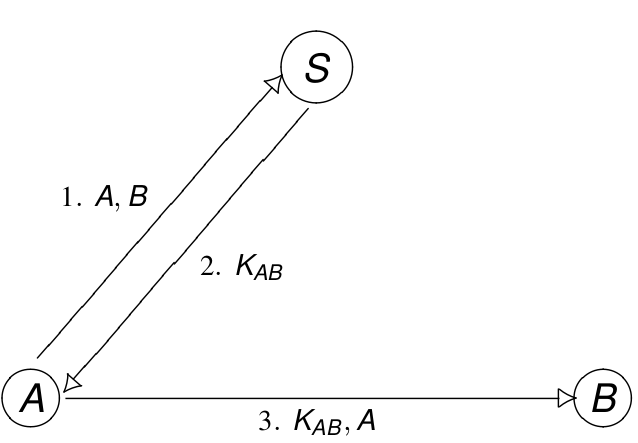
\includegraphics[width=.5\textwidth]{images/builtproto1}
\end{figure}
\noindent
Facciamo un primo tentativo, costruiamo un protocollo che consiste di tre passaggi:
\begin{enumerate}
	\item A contatta S inviandogli l'identificativo delle due entità che intendono condividere la chiave.
	\item S manda la chiave $K_{AB}$ ad A.
	\item A invia la chiave a B.
\end{enumerate}
Una rappresentazione equivalente alla figura è la seguente:
\begin{colbox}{beige}{4.5cm}
	\begin{enumerate}
		\item $\fromto{A}{S}A, B$
		\item $\fromto{S}{A}K_{AB}$
		\item $\fromto{A}{B}K_{AB},\,A$
	\end{enumerate}
\end{colbox}
NB: ``$A\rightarrow B\,$" serve a specificare sender e receiver, ma le identità A e B non sono parte del messaggio se non diversamente specificato.\\
In seguito utilizzaremo sempre questa nuova notazione.

Tornando al protocollo, notiamo un primo problema di notevole importanza: la chiave dev'essere comunicata solo ad A e B, nessun'altro deve poterla ricavare. Da ciò deriviamo la nostra prima \emph{security assumption}:
\begin{quote}
	\textbf{Security assumption 1}\\
	L'avversario è capace di origliare tutti i messaggi scambiati in un protocollo di sicurezza.
\end{quote}

\subsection{Secondo tentativo}
Sfruttiamo un algoritmo crittografico a chiave simmetrica per comunicare. Inizialmente S condivide con A la chiave $K_{AS}$ e con B la chiave $K_{BS}$.
\begin{colbox}{beige}{7cm}
	\begin{enumerate}
		\item $\fromto{A}{S}A, B$
		\item $\fromto{S}{A}\{K_{AB}\}_{K_{AS}},\ \{K_{AB}\}_{K_{BS}}$
		\item $\fromto{A}{B}\{K_{AB}\}_{K_{BS}},\ A$
	\end{enumerate}
\end{colbox}
In questo modo nessun avversario può leggere la chiave condivisa, ammesso sia valida la seguente assunzione.
\begin{quote}
	\textbf{Perfect cryptography assumption}\\
	I messaggi cifrati possono essere letti solo dai legittimi destinatari, i quali sono in possesso della chiave di decifratura.
\end{quote}
Tuttavia un avversario solitamente non è solo in grado di origliare i messaggi che passano sulla rete, bensì anche manipolarli.
\begin{quote}
	\textbf{Security assumption 2}\\
	L'avversario è capace di alterare tutti i messaggi usando qualsiasi informazione disponibile. Egli può inoltre reindirizzare messaggi ad altri principal (o semplicemente intercettarli) e generare messaggi completamente nuovi.
\end{quote}
Possiamo riassumere le prime due assunzioni di sicurezza come segue:
\begin{quote}
	\emph{L'avversario ha il completo controllo della rete.}
\end{quote}

\noindent Vediamo un paio di possibili attacchi man-in-the-middle.
\subsubsection{Man-in-the-middle tra A e B}
\begin{colbox}{beige}{7cm}
	\begin{enumerate}
		\item $\fromto{A}{S}A, B$
		\item $\fromto{S}{A}\{K_{AB}\}_{K_{AS}},\ \{K_{AB}\}_{K_{BS}}$
		\item $\fromto{A}{C}\{K_{AB}\}_{K_{BS}},\ A$
		\item $\fromto{C}{B}\{K_{AB}\}_{K_{BS}},\ D$
	\end{enumerate}
\end{colbox}
L'avversario C intercetta il messaggio di A e lo manipola per convincere B che il mittente del messaggio sia D (dove D può essere chiunque, compreso C stesso). La chiave rimane segreta, tuttavia questo metodo può essere sfruttato per un \emph{denial of service}.

\subsubsection{Man-in-the-middle tra A ed S}
\begin{colbox}{beige}{7cm}
	\begin{enumerate}
		\item $\fromto{A}{C}A, B$
		\item[$1'$.] $\fromto{C}{S}A, C$
		\item $\fromto{S}{C}\{K_{AC}\}_{K_{AS}},\ \{K_{AC}\}_{K_{CS}}$
		\item[$2'$.] $\fromto{C}{A}\{K_{AC}\}_{K_{AS}},\ \{K_{AC}\}_{K_{CS}}$
		\item $\fromto{A}{C}\{K_{AC}\}_{K_{CS}},\ A$
	\end{enumerate}
\end{colbox}
L'attaccante C altera il messaggio di A inviato ad S, chiedendo al server S di creare una chiave di sessione per A e C cifrata con chiave $K_{CS}$. A non può sapere se la chiave ottenuta è lecita o compromessa, e B non rileva alcuna anomalia in quanto C intercetta il messaggio originariamente rivolto a lui.

Questo è un attacco molto più pericoloso del precedente, in quanto C ora conosce la chiave e si è mascherato da B. Per funzionare tuttavia è necessario assumere che C sia un utente legittimo riconosciuto da S.
\begin{quote}
	\textbf{Security assumption 3}\\
	L'avversario può essere un utente legittimo (\emph{insider}), un entità esterna (\emph{outsider}) o una combinazione dei due.
\end{quote}

\subsection{Terzo tentativo}
Per impedire l'attacco di cui sopra, alleghiamo crittograficamente le identità dei principals alla chiave.
\begin{colbox}{beige}{7.5cm}
	\begin{enumerate}
		\item $\fromto{A}{S}A, B$
		\item $\fromto{S}{A}\{K_{AB},\,B\}_{K_{AS}},\ \{K_{AB},\,A\}_{K_{BS}}$
		\item $\fromto{A}{B}\{K_{AB}\}_{K_{BS}},\ A$
	\end{enumerate}
\end{colbox}
A questo punto l'attaccante non può compromettere il protocollo mediante intercettazione o alterazione di messaggi, a patto che A e B siano onesti.

Il protocollo non può ancora dirsi sicuro, infatti c'è una vulnerabilità che nasce dalla differenza di qualità tra le chiavi a lungo termine (scambiate con S) e le chiavi di sessione. Quest'ultime sono generate al fine di ottenere prestazioni migliori durante la comunicazione, ma aprono la strada a nuovi possibili attacchi: \emph{replay attack}.
\begin{quote}
	\textbf{Security assumption 4}\\
	L'avversario è capace di ricavare la chiave di sessione $K_{AB}$ usata in scambi di messaggi ``sufficientemente vecchi".
\end{quote}

\subsubsection{Replay attack}
\begin{colbox}{beige}{7cm}
	\begin{enumerate}
		\item $\fromto{A}{C}A, B$
		\item $\fromto{C}{A}\{K_{AB}'\}_{K_{AS}},\ \{K_{AB}'\}_{K_{BS}}$
		\item $\fromto{A}{B}\{K_{AB}'\}_{K_{BS}},\ A$
	\end{enumerate}
\end{colbox}
L'attaccante intercetta il messaggio di A rivolto al server S, il quale non ha alcun ruolo in questo attacco. Nelle veci del server, C invia ad A una chiave di sessione $K_{AB}'$ già usata in passato, perciò già ricavata da C.

Alla fine del protocollo, A e B condivideranno la chiave compromessa $K_{AB}'$, perciò C potrà leggere ed eventualmente modificare qualcunque messaggio scambiato tra i due principals.
\emph{Come possiamo prevenirlo?}

Metodo del \textbf{challenge-response}: uno dei principal genera e invia un \emph{nonce} (``number used only once"), ovvero sceglie un numero casualmente. Quest'ultimo viene ritornato al mittente per verificare che il messaggio sia generato ex-novo.

\subsection{Protocollo di Needham-Schroeder}\label{sec:NSSK}
\begin{colbox}{beige}{8.5cm}
	\begin{enumerate}
		\item $\fromto{A}{S}A, B, N_A$
		\item $\fromto{S}{A}\{K_{AB},B,N_A,\{K_{AB},A\}_{K_{BS}}\}_{K_{AS}}$
		\item $\fromto{A}{B}\{K_{AB},A\}_{K_{BS}}$
		\item $\fromto{B}{A}\{N_B\}_{K_{AB}}$
		\item $\fromto{A}{B}\{N_B-1\}_{K_{AB}}$
	\end{enumerate}
\end{colbox}

Nel protocollo di Needham-Schroeder, il nonce $N_A$ inviato da A e ritornato da S permette di assicurare non solo la \emph{freshness} del pacchetto per A, ma anche quella del pacchetto per B siccome è cifrato nello stesso messaggio. Non avremmo ottenuto le stesse proprietà di sicurezza se il secondo messaggio fosse stato il seguente:
\begin{equation*}
	2.\ S\rightarrow A\!:\ \{K_{AB},B,N_A\}_{K_{AS}},\ \{K_{AB},A\}_{K_{BS}}
\end{equation*}
I messaggi 4 e 5 consistono in un ulteriore handshake tra A e B per assicurare il secondo principal della freshness della chiave $K_{AB}$.\\
NB: \emph{i nonce sono semplici numeri}, non contengono indizi riguardo l'identità del principal che li ha generati.\\

Il protocollo di Needham-Schroeder è vulnerabile ad un attacco man-in-the-middle conosciuto come attacco di \emph{Denning and Sacco}.

\subsubsection{Denning and Sacco attack}
Questo attacco man-in-the-middle si basa su una vulnerabilità del protocollo Needham-Schroeder, secondo il quale nessuno a parte A sia in grado di rispondere alla challenge di B del quarto messaggio. Per la quarta security assumption, sappiamo che un avversario C potrebbe conoscere una vecchia chiave di sessione $K_{AB}'$. C potrebbe dunque fingersi A e persuadere B a usare la chiave di sessione di cui è a conoscenza.
\begin{colbox}{beige}{5.5cm}
	\begin{enumerate}
		\item[3.] $\fromto{C}{B}\{K_{AB}',A\}_{K_{BS}}$
		\item[4.] $\fromto{B}{C}\{N_B\}_{K_{AB}'}$
		\item[5.] $\fromto{C}{B}\{N_B-1\}_{K_{AB}'}$
	\end{enumerate}
\end{colbox}

\subsection{Quinto (e ultimo) tentativo}
Affinché il protocollo non sia vulnerabile ai replay attack, sia A che B devono inviare una challenge a S.
\begin{colbox}{beige}{9cm}
	\begin{enumerate}
		\item $\fromto{B}{A}B,N_B$
		\item $\fromto{A}{S}A,B,N_A,N_B$
		\item $\fromto{S}{A}\{K_{AB},B,N_A\}_{K_{AS}},\ \{K_{AB},A,N_B\}_{K_{BS}}$
		\item $\fromto{A}{B}\{K_{AB},A,N_B\}_{K_{BS}}$
	\end{enumerate}
\end{colbox}
Questa volta la comunicazione viene iniziata da B, il quale invia il proprio nonce ad A. Quest'ultimo comunica con il server che gli risponde con le chiavi di sessione separate, ognuna contenuta nella rispettiva response per garantire la freshness.

Può sembrare di aver ottenuto più proprietà con meno scambi di messaggi, a differenza del quarto tentativo abbiamo in realtà perso la proprietà di \emph{key confirmation}: al termine del protocollo non sappiamo con certezza se B è a conoscenza della chiave.

La versione finale di questo protocollo non è vulnerabile ad alcun attacco tra quelli visti fino ad ora, tuttavia è presto per poter affermare che il protocollo è \emph{sicuro}, dobbiamo prima dare una definizione formale degli obiettivi che deve soddisfare.

\subsection{Security assumptions}
Riassumiamo le assunzioni di sicurezza:
\begin{enumerate}
	\item[0.] (\emph{Perfect cryptography assumption}) I messaggi cifrati possono essere letti solo dai legittimi destinatari, i quali sono in possesso della chiave di decifratura.
	\item L'avversario è capace di origliare tutti i messaggi scambiati in un protocollo di sicurezza.
	\item L'avversario è capace di alterare tutti i messaggi usando qualsiasi informazione disponibile. Egli può inoltre reindirizzare messaggi ad altri principal (o semplicemente intercettarli) e generare messaggi completamente nuovi.
	\item L'avversario può essere un utente legittimo (\emph{insider}), un entità esterna (\emph{outsider}) o una combinazione dei due.
	\item L'avversario è capace di ricavare la chiave di sessione $K_{AB}$ usata in scambi di messaggi ``sufficientemente vecchi".
\end{enumerate}

\clearpage
\section{Needham-Schroeder Public Key}
Studiamo il protocollo Needham-Schroeder Public Key (NSPK), che mira a garantire l'autenticazione dei principal:
\begin{colbox}{beige}{5cm}
	\begin{enumerate}
		\item $\fromto{A}{B}\{N_A,A\}_{K_B}$
		\item $\fromto{B}{A}\{N_A,N_B\}_{K_A}$
		\item $\fromto{A}{B}\{N_B\}_{K_B}$
	\end{enumerate}
\end{colbox}
NB: è omessa l'interazione con il server per chiedere le chiavi pubbliche.\\
Obiettivi del protocollo:
\begin{itemize}
	\item \emph{Autenticazione} dei messaggi.
	\item \emph{Timeliness}, ovvero freshness dei messaggi.
	\item \emph{Segretezza}, se fossero violati i nonce potrebbe fallire l'autenticazione.
\end{itemize}

\noindent
Modello dell'attaccante: questi conosce il protocollo ma non può rompere la crittografia, inoltre può essere \emph{attivo} o \emph{passivo} se rispettivamente interviene nella conversazione o se ascolta solamente.

\textbf{Dolev-Yao attacker}: modello standard di attaccante, molto potente in quanto ha il pieno controllo della rete, senza tuttavia invalidare l'assunzione di perfect cryptography.

\subsection{Lowe attack}
L'attacco di Lowe a NSPK è un man-in-the-middle in cui A vuole comunicare con C, ma quest'ultimo ha intenzioni malevole e vuole fingersi A per comunicare con B.
\begin{colbox}{beige}{5cm}
	\begin{enumerate}
		\item $\fromto{A}{C}\{N_A,A\}_{K_C}$
		\item $\fromto{C}{B}\{N_A,A\}_{K_B}$
		\item $\fromto{B}{C}\{N_A,N_B\}_{K_A}$
		\item $\fromto{C}{A}\{N_A,N_B\}_{K_A}$
		\item $\fromto{A}{C}\{N_B\}_{K_C}$
		\item $\fromto{C}{B}\{N_B\}_{K_B}$
	\end{enumerate}
\end{colbox}
Protocollo Needham-Schroeder-Lowe (NSL): nella risposta B invia la propria identità, oltre ai nonce.
\begin{colbox}{beige}{5.5cm}
	\begin{enumerate}
		\item $\fromto{A}{B}\{N_A,A\}_{K_B}$
		\item $\fromto{B}{A}\{N_A,N_B,B\}_{K_A}$
		\item $\fromto{A}{B}\{N_B\}_{K_B}$
	\end{enumerate}
\end{colbox}

\subsection{Type-flaw attack}
In un type-flaw attack un principal viene ingannato riguardo il tipo di dato che riceve: l'attaccante invia al principal un messaggio con il giusto numero di bit, ma il cui contenuto è di tipo diverso. Questo attacco è inoltre un \emph{oracle attack}, in quanto la vittima, seguendo il protocollo, invia all'attaccante informazioni utili per proseguire nell'attacco.

\begin{figure}[htp]
	\centering
	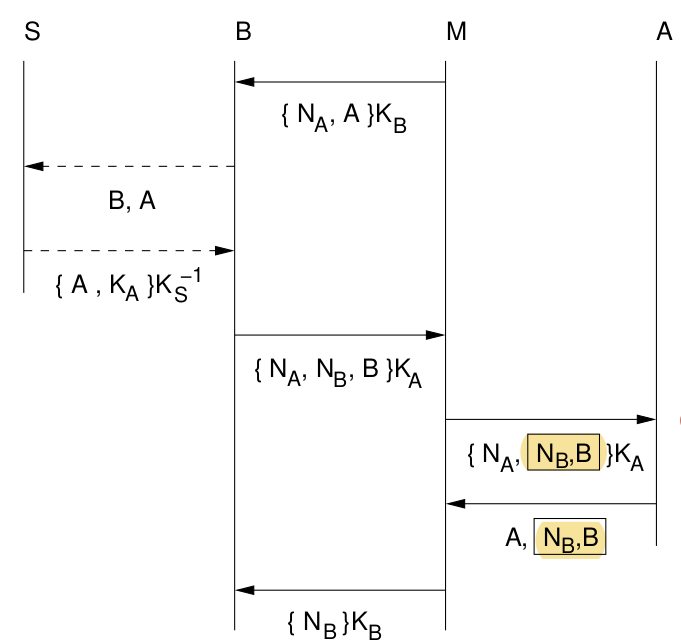
\includegraphics[width=.8\textwidth]{images/OracleAttack}
	\caption{Oracle attack da parte dell'attaccante M.}\label{fig:oracle}
\end{figure}
\noindent In figura [\ref{fig:oracle}] vediamo come l'attaccante M (man-in-the-middle) intenda fingersi A nella comunicazione con B. Per riuscire nel suo intento, M manda a B il primo messaggio del protocollo NSL indicando A come mittente. Quando B risponde con un messaggio cifrato con la chiave pubblica di A, M lo rigira ad A come fosse il primo messaggio del protocollo. A quindi interpreterà (erroneamente) il tipo del messaggio e cercherà di contattare S chiedendo una chiave per comunicare con "$N_B,B$". M intercetterà quest'ultimo messaggio e potrà rispondere infine a B per aprire una comunicazione fingendosi A.\\
Versione definitiva, che fa uso di firme digitali per evitare type-flaw attack:
\begin{colbox}{beige}{6cm}
	\begin{enumerate}
		\item $\fromto{A}{B}\{[N_A,A]_{K_A^{-1}}\}_{K_B}$
		\item $\fromto{B}{A}\{N_A,[N_B]_{K_B^{-1}}\}_{K_A}$
		\item $\fromto{A}{B}\{[N_B]_{K_A^{-1}}\}_{K_B}$
	\end{enumerate}
\end{colbox}

\section{Tipi di attacco}
Elenchiamo i principali tipi di attacco, per poi vedere esempi di protocolli con relative vulnerabilità:
\begin{enumerate}
	\item \emph{Man-in-the-middle}\\
	L'attaccante si posiziona in mezzo a due principal, intercettandone i messaggi per invalidare il protocollo: $A \leftrightarrow Z \leftrightarrow B$.
	\item \emph{Parallel session}\\
	Man-in-the-middle in cui l'attaccante sfrutta più run del protocollo contemporaneamente.
	\item \emph{Replay}\\
	L'attaccante riusa parti di messaggi precedenti come fossero fresh.
	\item \emph{Masquerading}\\
	L'attaccante finge di essere un altro principal.
	\item \emph{Reflection}\\
	Alcune informazioni vengono ritrasmesse al mittente.
	\item \emph{Oracle}\\
	Istanziando un protocollo con terzi principal, l'avversario può sfruttare le risposte legittime al protocollo per fare encryption/decryption di messaggi.
	\item \emph{Type-flaw}\\
	L'attaccante sostituisce campi del messaggio con informazioni di altro genere, senza invalidare la formattazione del messaggio stesso.
\end{enumerate}

\subsection{Otway-Rees protocol}
Protocollo server-based per la distribuzione autenticata di chiavi, che garantisce segretezza e freshness delle chiavi, senza però assicurare autenticazione dei principal e key-confirmation.
\begin{colbox}{beige}{10cm}
	\begin{enumerate}
		\item $\fromto{A}{B}I,A,B,\{N_A,I,A,B\}_{K_{AS}}$
		\item $\fromto{B}{S}I,A,B,\{N_A,I,A,B\}_{K_{AS}},\{N_B,I,A,B\}_{K_{BS}}$
		\item $\fromto{S}{B}I,\{N_A,K_{AB}\}_{K_{AS}},\{N_B,K_{AB}\}_{K_{BS}}$
		\item $\fromto{B}{A}I,\{N_A,K_{AB}\}_{K_{AS}}$
	\end{enumerate}
\end{colbox}
In questo caso, $I$ è l'identificativo della run del protocollo.\\
Vediamo due possibili vulnerabilità del protocollo Otway-Rees:
\begin{itemize}
	\item \emph{Reflection/Type-flaw}\\
	Supponendo $|\{I,A,B\}=\{K_{AB}\}|$, un attaccante Z potrebbe intercettare il primo messaggio e, fingendosi B, rispondere ad A con $I,\{N_A,I,A,B\}_{K_{AS}}$. A vede che il nonce è corretto, perciò accetta $\{I,A,B\}$ come chiave di sessione.
	\item In modo analogo al precedente attacco, Z si maschera da server S e risponde a B ``riflettendo" le parti cifrate dei primi messaggi.
	\begin{equation*}
		3.\ \fromto{Z}{B}I,\{N_A,I,A,B\}_{K_{AS}},\{N_B,I,A,B\}_{K_{BS}}
	\end{equation*}
	In questo modo Z può leggere e manipolare la comunicazione tra A e B, invalidando key-authentication e segretezza.
\end{itemize}

\subsection{Andrew Secure RCP protocol}
In questo protocollo, due principal che condividono una chiave simmetrica $K_{AB}$ intendono scambiarsi una nuova chiave condivisa $K_{AB}'$ che sia autenticata, fresh e segreta.
\begin{colbox}{beige}{6cm}
	\begin{enumerate}
		\item $\fromto{A}{B}A,\{N_A\}_{K_{AB}}$
		\item $\fromto{B}{A}\{N_A+1,N_B\}_{K_{AB}}$
		\item $\fromto{A}{B}\{N_B+1\}_{K_{AB}}$
		\item $\fromto{B}{A}\{K_{AB}',N_B'\}_{K_{AB}}$
	\end{enumerate}
\end{colbox}
\emph{Type-flaw attack}
Un attaccante Z può fare man-in-the-middle fingendosi B, intercettando il terzo messaggio e rimandando ad A il secondo come quarto messaggio:
\begin{equation*}
	4.\ \fromto{Z}{A}\{N_A+1,N_B\}_{K_{AB}}
\end{equation*}
Al termine dell'attacco A accetta come nuova chiave di sessione $N_A+1$, che non è autenticata. In questo caso la secrecy non è stata violata.

\subsection{Key exchange with CA}
Questo protocollo, conosciuto anche come ``Denning \& Sacco", permette a due principal in possesso di una chiave di sessione di scambiarsi il certificati di autenticazione. Aggiungiamo alcuni elementi alla notazione: $C_A$ indica il certificato di A, $T_A$ indica un timestamp generato da A. In questo caso inoltre S rappresenta il server di una CA.
\begin{colbox}{beige}{7.5cm}
	\begin{enumerate}
		\item $\fromto{A}{S}A,B$
		\item $\fromto{S}{A}C_A,C_B$
		\item $\fromto{A}{B}C_A,C_B,\{\{T_A,K_{AB}\}_{K_A^{-1}}\}_{K_B}$
	\end{enumerate}
\end{colbox}
Un attacco a questo protocollo si presenta quando A vuole comunicare con Z, ma Z usa il messaggio ricevuto per contattare B fingendosi A:
\begin{gather*}
	\fromto{A}{Z}C_A,C_Z,\{\{T_A,K_{AZ}\}_{K_A^{-1}}\}_{K_Z}\\
	\fromto{Z}{B}C_A,C_B,\{\{T_A,K_{AZ}\}_{K_A^{-1}}\}_{K_B}
\end{gather*}
Giunti a questo punto, B crede di comunicare con A, invece parla con Z: sono state invalidate sia l'autenticazione che la segretezza. Come difendersi?\\
Nell'ultimo messaggio vanno specificati anche i principal interessati:
\begin{equation*}
	3.\ \fromto{A}{B}C_A,C_B,\{\{A,B,T_A,K_{AB}\}_{K_A^{-1}}\}_{K_B}
\end{equation*}

\subsection{Esempi di attacco}
Vediamo qualche esempio di attacco: binding, parallel session e replay.

\subsubsection{Binding attack}
Il seguente protocollo:
\begin{colbox}{beige}{6.5cm}
	\begin{enumerate}
		\item $\fromto{A}{S}A,B,N_A$
		\item $\fromto{S}{A}S,\{S,A,N_A,K_B\}_{K_S^{-1}}$
	\end{enumerate}
\end{colbox}
ammette un \emph{binding attack}:
\begin{colbox}{beige}{6.5cm}
	\begin{enumerate}
		\item[1.1.] $\fromto{A}{Z}A,B,N_A$
		\item[2.1.] $\fromto{Z}{S}A,Z,N_A$
		\item[2.2.] $\fromto{S}{Z}S,\{S,A,N_A,K_Z\}_{K_S^{-1}}$
		\item[1.2.] $\fromto{Z}{A}S,\{S,A,N_A,K_Z\}_{K_S^{-1}}$
	\end{enumerate}
\end{colbox}
In questo caso Z si spaccia per B nella comunicazione.\\
Fix: aggiungiamo l'identità del destinatario B nel secondo messaggio.
\begin{equation*}
	2.\ \fromto{S}{A}S,\{S,A,N_A,B,K_B\}_{K_S^{-1}}
\end{equation*}

\subsubsection{Parallel session attack}
Il seguente protocollo one-way di autenticazione:
\begin{colbox}{beige}{5cm}
	\begin{enumerate}
		\item $\fromto{A}{B}\{N_A\}_{K_{AB}}$
		\item $\fromto{B}{A}\{N_A+1\}_{K_{AB}}$
	\end{enumerate}
\end{colbox}
ammette un \emph{parallel-session attack} con ``oracle":
\begin{colbox}{beige}{5cm}
	\begin{enumerate}
		\item[1.1.] $\fromto{A}{Z}\{N_A\}_{K_{AB}}$
		\item[2.1.] $\fromto{Z}{B}\{N_A\}_{K_{AB}}$
		\item[2.2.] $\fromto{A}{Z}\{N_A+1\}_{K_{AB}}$
		\item[1.2.] $\fromto{Z}{A}\{N_A+1\}_{K_{AB}}$
	\end{enumerate}
\end{colbox}
A è costretto ad agire da oracolo contro se stesso, fornendo a Z la risposta alla propria stessa challenge. L'attaccante quindi, sfruttando due sessioni dello stesso protocollo, riesce ad autenticarsi mascherato da B.\\
Fix: aggiungiamo l'identità del mittente A al primo messaggio.
\begin{equation*}
	1.\ \fromto{A}{B}\{N_A,A\}_{K_{AB}}
\end{equation*}

\subsubsection{Replay attack}
Il protocollo Needham-Schroeder Shared Key ammette un \emph{replay attack}, vedi sezione [\ref{sec:NSSK}].

\subsection{Buone norme per protocolli di sicurezza}
\begin{itemize}
	\item Ogni messaggio deve contenere tutto il necessario (incluse le identità dei principal).
	\item Dev'essere chiaro perché determinati meccanismi crittografici vengono applicati.
	\item Dev'essere chiaro perché vengono sfruttati i nonce.
	\item Tener conto di possibili replay-attack approfittando di challenge-response.
	\item Devono essere chiare le relazioni di fiducia tra i principal.
\end{itemize}


\chapter{Protocolli di sicurezza moderni}
%TODO In quali layer implementiamo la sicurezza (slide 86 img figa)
\section{Kerberos}
Protocollo per l'autenticazione ed il controllo degli accessi in ambienti aperti e distribuiti. Il nome del protocollo è dovuto all'intezione di implementare una proprietà per ogni testa di Cerbero: autenticazione, accounting e auditing. \`E stata realizzata solo la prima.\\
Caratteristiche di Kerberos:
\begin{itemize}
	\item \emph{Sicuro}\\
	Nessun attaccante può impersonare un utente del sistema.
	\item \emph{Affidabile}\\
	I servizi offerti da Kerberos devono essere sempre fruibili da tutti i programmi dell'architettura distribuita.
	\item \emph{Trasparente}\\
	Deve prevedere un meccanismo di \emph{single sign-on} (SSO), affinché l'utente possa usare un'unica password per tutti i servizi offerti.
	\item \emph{Scalabile}\\
	Il sistema dev'essere scalabile per supportare un vasto numero di utenti.
\end{itemize}
L'architettura di Kerberos si compone di due server: il \emph{Kerberos Authentication Server} (KAS) ed il \emph{Ticket Granting Server} (TGS). Inoltre è presente un controllo degli accessi per controllare i ticket emessi dal TGS.

\begin{figure}[htp]
	\centering
	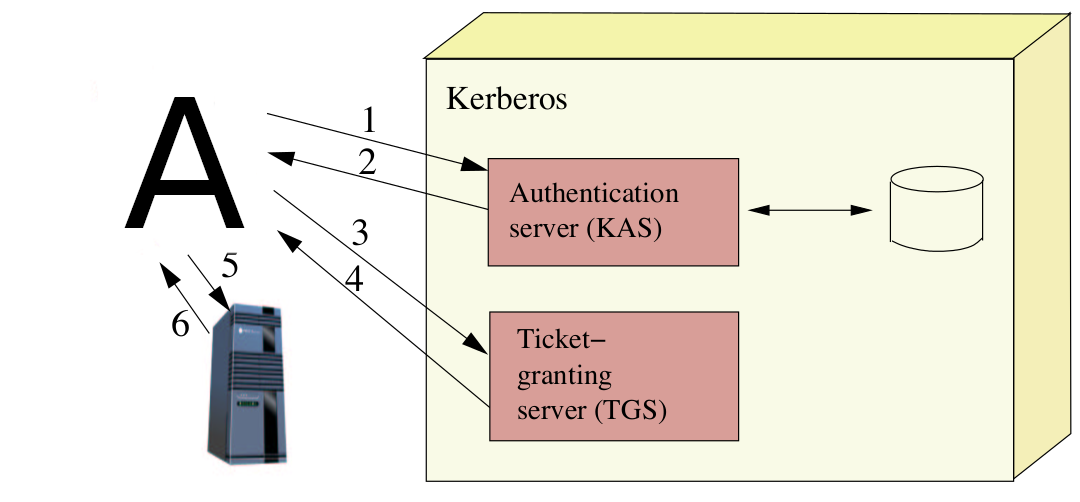
\includegraphics[width=.9\textwidth]{images/kerberos}
	\caption{Architettura di Kerberos.}
\end{figure}

\subsection{Funzionamento}
Il funzionamento di Kerberos si divide in tre fasi basate su Needham-Schroeder, usando tuttavia i timestamps al posto dei nonce per garantire freshness.
\begin{itemize}
	\item Autenticazione dell'utente.
	\item Autorizzazione per l'uso di un certo servizio.
	\item Connessione al servizio.
\end{itemize}
La fase di autenticazione viene svolta al login, in seguito alla quale l'utente è autenticato per svariate ore (la durata dipende all'applicazione):
\begin{colbox}{beige}{12cm}
	\begin{enumerate}
		\item $\fromto{A}{KAS}A,TGS$
		\item $\fromto{KAS}{A}\{K_{A,T\!G\!S},TGS,T_1,
		\underbrace{\{A,TGS,K_{A,T\!G\!S},T_1\}_{K_{K\!A\!S,T\!G\!S}}}_{\mbox{Authentication Ticket}}\}_{K_{AS}}$
	\end{enumerate}
\end{colbox}
L'utente A vuole eseguire il login, perciò KAS accede al database e invia ad A una chiave di sessione $K_{A,TGS}$ ed un \emph{Authentication Ticket} cifrato.
La validità della chiave di sessione è legata al timestamp $T_1$. L'intero messaggio è cifrato con chiave $K_{AS}$, che deriva dalla password dell'utente.

Per accedere ad un servizio B, A deve presentare l'auth ticket ricevuto al login insieme ad un \emph{Authenticator}:
\begin{colbox}{beige}{12cm}
	\begin{enumerate}
		\item[3.] $\fromto{A}{TGS}\underbrace{\{A,TGS,K_{A,T\!G\!S},T_1\}_{K_{K\!A\!S,T\!G\!S}}}_{\mbox{Auth Ticket}}, \underbrace{\{A,T_2\}_{K_{A,T\!G\!S}}}_{\mbox{Authenticator}}, B$
		\item[4.] $\fromto{TGS}{A}\{K_{A,B},B,T_3,\underbrace{\{A,B,K_{A,B},T_3\}_{K_{B,T\!G\!S}}}_{\mbox{Service Ticket}}\}_{K_{A,T\!G\!S}}$
	\end{enumerate}
\end{colbox}
Questa fase dev'essere svolta ogni volta che A vuole accedere ad un servizio B. Inoltre il timestamp $T_2$ ha un lifetime di pochi secondi per prevenire replay attacks; il server tiene traccia dei recenti authenticators per prevenire replay immediati. Nel quarto messaggio, il TGS invia ad A una nuova chiave di sessione $K_{A,B}$ con validità di pochi minuti ed un \emph{Service Ticket}.

Nella terza ed ultima fase, A contatta il servizio B fornendo il service ticket ed un nuovo authenticator cifrato con la chiave di sessione:
\begin{colbox}{beige}{10cm}
	\begin{enumerate}
		\item[5.] $\fromto{A}{B}\underbrace{\{A,B,K_{A,B},T_3\}_{K_{B,T\!G\!S}}}_{\mbox{Service Ticket}}, \underbrace{\{A,T_4\}_{K_{A,B}}}_{\mbox{Authenticator}}$
		\item[6.] $\fromto{B}{A}\{T_4+1\}_{K_{A,B}}$
	\end{enumerate}
\end{colbox}
Il sesto messaggio (opzionale) conferma l'accesso di A al servizio B.

\subsection{Scalabilità}
Kerberos risulta altamente scalabile grazie alla suddivisione dei servizi in \emph{reami}. Ogni reame è definito e gestito da un server Kerberos, il cui TGS conosce i servizi del proprio reame e il TGS dei servizi esterni. Nel caso un utente A volesse accedere ad un servizio B di un altro reame, il TGS di A lo indirizzerebbe al server corretto fornendogli una chiave per contattarlo (fase 2 svolta due volte).

\subsection{Limitazioni della versione IV}
\begin{itemize}
	\item Sfruttanto il primo messaggio, un attaccante potrebbe fare \emph{flooding} contro il KAS, con conseguente DoS.
	\item La doppia cifratura nel secondo messaggio è ridondante (eliminata nella versione V).
	\item La difesa dai replay attack dipende eccessivamente dai timestamp, se l'utente è compromesso tali attacchi risultano possibili.
\end{itemize}
Alcune di queste limitazioni sono tuttora riscontrabili nella versione V.


\section{TLS/SSL}
\emph{Secure Sockets Layer} e \emph{Transport Layer Security} sono protocolli di sicurezza per il livello di trasporto, non sono gestiti dal sistema operativo ma dall'applicazione. Sono lo stesso protocollo, ma sfruttano algoritmi crittografici diversi (TLS è successivo a SSL ed è stato standardizzato nel 1999).
L'obiettivo di TSL/SSL è garantire privacy e integrità dei dati tra due applicazioni che comunicano (\emph{end-to-end}), anche in presenza di attacchi via rete.

SSL consiste di due protocolli: uno di handshake e uno di record. Il primo utilizza la crittografia a chiave asimmetrica per stabilire diverse chiavi di sessione, il secondo sfrutta le chiavi generate per garantire confidenzialità, integrità e autenticità durante la comunicazione tra client e server.

\subsection{Handshake}
\begin{minipage}{.65\textwidth}
	L'handshake prevede la negoziazione sulla versione del protocollo da usare e l'autenticazione facoltativa di client e server mediante certificati digitali.\\
	Il protocollo si suddivide in 4 fasi:
	\begin{enumerate}
		\item Negoziazione delle versioni del protocollo.
		\item Scambio del certificato del server.
		\item Scambio della chiave del client.
		\item Instaurazione della connessione.
	\end{enumerate}
\end{minipage}
\begin{minipage}{.35\textwidth}
	\centering
	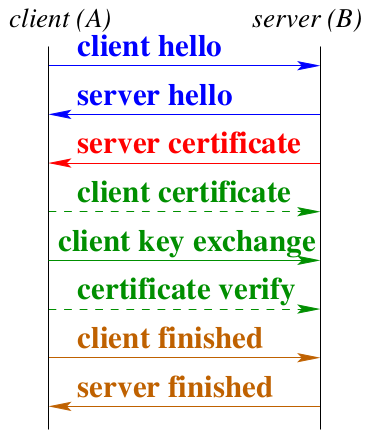
\includegraphics[width=.95\textwidth]{images/SSL}
\end{minipage}

\clearpage
\begin{enumerate}
	\item[Fase 1.] \emph{Hello}
	\begin{colbox}{beige}{6cm}
		\begin{enumerate}
			\item[1.] $\fromto{A}{B}A,N_A,SID,P_A$
			\item[2.] $\fromto{B}{A}N_B,SID,P_B$
		\end{enumerate}
	\end{colbox}
	A identifica il client (in pratica, l'IP nel protocollo TCP).
	B identifica il server.
	SID è il \emph{Session Identifier}.
	$P_A$ indica le preferenze di A riguardo gli algoritmi di cifratura e compressione. Il server mette in $P_B$ gli algoritmi più sicuri tra quelli supportati da A.
	\item[Fase 2.] \emph{Server certificate}
	\begin{colbox}{beige}{6cm}
		\begin{enumerate}
			\item[3.] $\fromto{B}{A}\mbox{\emph{certificate}}(B,K_B)$
		\end{enumerate}
	\end{colbox}
	Il server B invia ad A il proprio certificato, in formato X.509v3, firmato da un entità trusted.
	\item[Fase 3.] \emph{Client exchange}
	\begin{colbox}{beige}{6cm}
		\begin{enumerate}
			\item[4.] $\fromto{A}{B}\mbox{\emph{certificate}}(A,K_A)$
			\item[5.] $\fromto{A}{B}\{PMS\}_{K_B}$
			\item[6.] $\fromto{A}{B}\{\mbox{\emph{hash}}(\dots)\}_{K_A^{-1}}$
		\end{enumerate}
	\end{colbox}
	PMS è il \emph{pre-master secret}, usato in seguito per generare un \emph{master secret} $M$:
	\begin{equation*}
		M = PRF(PMS, N_A, N_B)
	\end{equation*}
	dove PRF è una Pseudo-Random Function (hash).\\
	Il quarto ed il sesto messaggio sono opzionali e raramente richiesti, servono per autenticare il client. Nel senso A invia l'hash computato usando tutti i messaggi precedenti.
	\item[Fase 4.] \emph{Finish}
	\begin{colbox}{beige}{6cm}
		\begin{enumerate}
			\item[7.] $\fromto{A}{B}\{\mbox{\emph{Finished}}\}_{\mbox{\emph{clientK}}}$
			\item[8.] $\fromto{B}{A}\{\mbox{\emph{Finished}}\}_{\mbox{\emph{serverK}}}$
		\end{enumerate}
	\end{colbox}
	\emph{Finished} è l'hash dei messaggi precedenti, usato per impedire \emph{downgrading attack} sugli algoritmi di cifratura.
	\emph{clientK} e \emph{serverK} sono chiavi simmetriche generate da $N_A,\ N_B$ ed $M$.
\end{enumerate}

\subsection{Gestione delle chiavi private}
I metodi per mantenere le chiavi private protette nel server sono:
\begin{itemize}
	\item Sfruttare hardware ad-hoc.
	\item Mantenere le chiavi cifrate (serve una password ad ogni reboot).
	\item Mantenere le chiavi in chiaro.
\end{itemize}
Ad oggi la metodologia più utilizzata è la terza.

\section{IPsec}
Il protocollo \emph{IPsec} nasce in quanto il protocollo IP non prevede meccanismi di sicurezza. Esso fornisce un canale sicuro per ogni applicazione, garantendo confidenzialità (cifratura dei dati), integrità (checksum) e autenticazione (firme e certificati). Dev'essere installato sul sistema operativo, o sui security gateway per implementare \emph{Virtual Private Networks} (VPNs).

Per evitare di rallentare inutilmente le comunicazioni, IPsec non viene usato nelle reti locali, ma solo nel trasporto di pacchetti via internet.
\begin{figure}[htp]
	\centering
	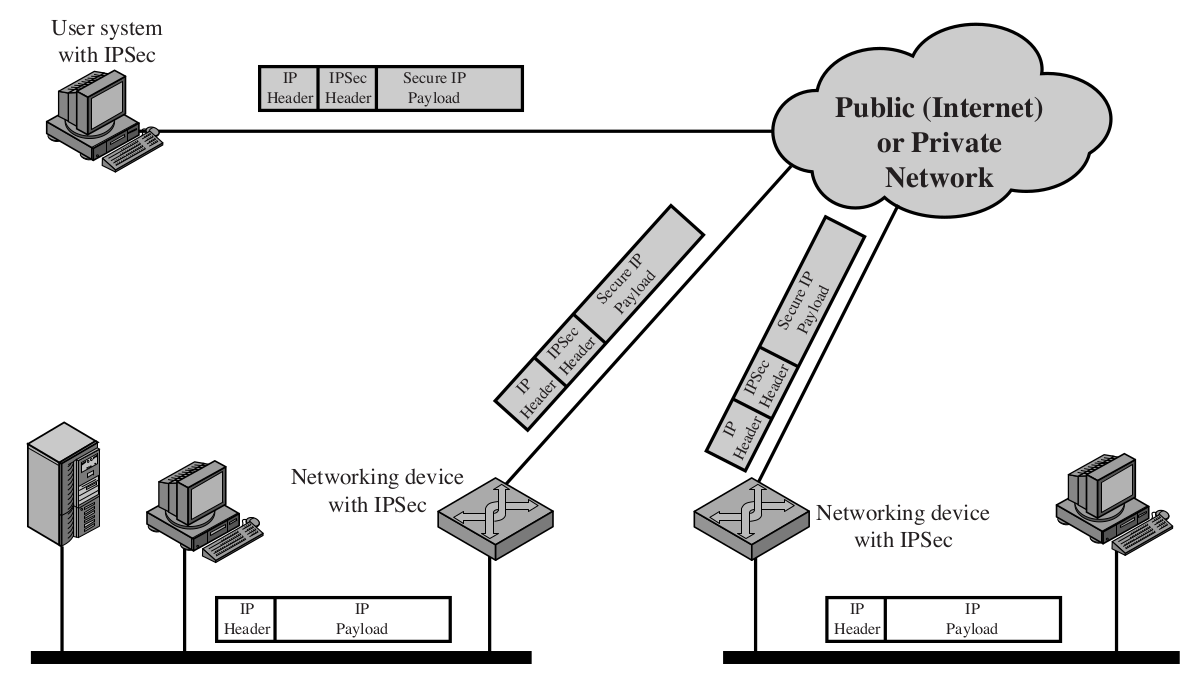
\includegraphics[width=\textwidth]{images/IPsecScenario}
	\caption{Un possibile scenario di IPsec.}
\end{figure}

\noindent
IPsec si compone di tre diversi protocolli:
\begin{itemize}
	\item \emph{Authentication Header} (AH)\\
	Garantisce l'autenticazione (in seguito inglobato da ESP).
	\item \emph{Encapsulatin Secuity Payload} (ESP)\\
	Garantisce confidenzialità e integrità.
	\item \emph{Key Management} (IKE)\\
	Gestisce lo scambio di chiavi.
\end{itemize}
IPsec prevede due modalità di utilizzo: \emph{Tunnel mode} e \emph{Transport mode}. Nella prima modalità il pacchetto originale viene completamente cifrato e inserito in un nuovo pacchetto IP, il quale ha un nuovo header IP e un header IPsec. Tale meccanismo è comunemente utilizzato nelle VPN. Nella transport mode viene cifrato il payload e aggiunto un header IPsec, mantenendo l'originale header IP (vedi fig. [\ref{fig:tunneltransport}]).
\begin{figure}[htp]
	\centering
	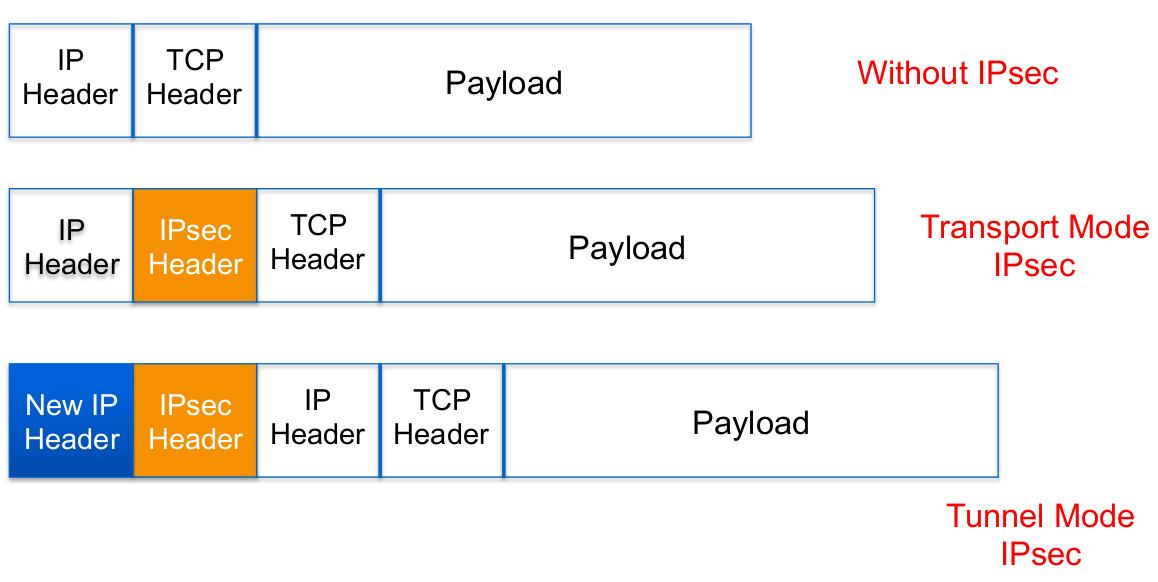
\includegraphics[width=.9\textwidth]{images/TunnelTransport}
	\caption{Tunnel mode e Transport mode di IPsec.}\label{fig:tunneltransport}
\end{figure}

\subsection{Authentication Header}
\begin{figure}[htp]
	\centering
	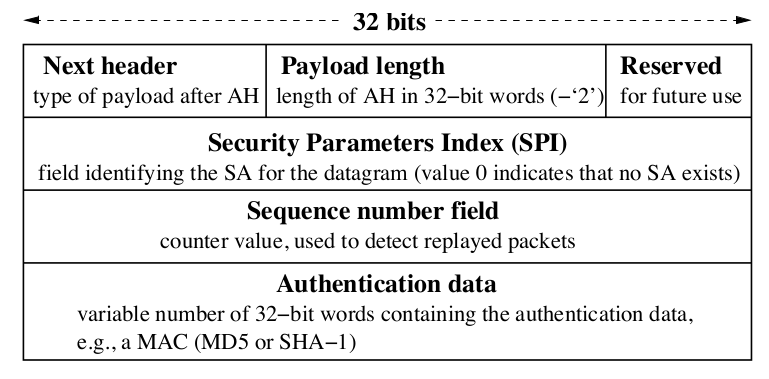
\includegraphics[width=.8\textwidth]{images/AH}
	\caption{Authentication Header (AH).}
\end{figure}
L'header di IPsec si colloca tra l'header IP ed il layer di trasporto, contiene un \emph{sequence number} per evitare replay attack e un campo relativo all'\emph{authentication data} che identifica la comunicazione. Per poter funzionare inoltre, IPsec genera mediante IKE delle \emph{Security Associations} (SA), le quali sono relazioni one-way tra mittente e destinatario. Una SA permette di specificare algoritmi per autenticazione e cifratura, chiavi, lifetime delle chiavi, protocol-mode (tunnel/transport). L'identificativo della SA è contenuto nel campo \emph{Security Parameters Index} (SPI) dell'AH.

\subsection{Encapsulating Security Payload}
Il protocollo ESP si occupa di cifrare e, opzionalmente, autenticare il messaggio. Per garantire confidenzialità, cifra il payload e aggiunge in testa un header contenente le informazioni per la corretta decifratura. L'autenticazione è ottenuta invece aggiungendo in coda al pacchetto un MAC ottenuto dall'hash dei precedenti campi.

Usando sia AH che ESP enll'header IPsec possiamo garantire confidenzialità, integrità, autenticazione e difesa da replay attack.
\begin{figure}[htp]
	\centering
	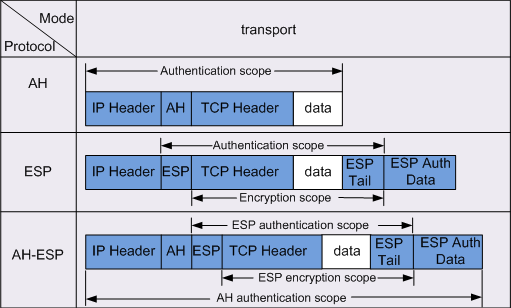
\includegraphics[width=.95\textwidth]{images/IPsecHeader}
	\caption{IPsec header}
\end{figure}

\subsection{Internet Key Exchange}
La gestione delle chiavi è delegata ad IKE, un protocollo flessibile ma complesso che permette di stabilire SA. IKE nasce come evoluzione di diversi protocolli basati su Diffie-Hellman, al quale aggiunge l'autenticazione mantenendo la \emph{Perfect Forward Secrecy} (PFS), proprietà che garantisce la segretezza della sessione anche dopo la rottura della chiave long-term.

Il protocollo prevede due fasi, dette \emph{Main mode} e \emph{Quick mode}, di cui la prima è usata solo nel caso i due principal non si conoscano. Nella main viene stabilita la SA per la fase successiva, durante la quale vengono create delle SAs figlie per cifrare e autenticare le future comunicazioni.\\
Main mode:
\begin{colbox}{beige}{7.5cm}
	\begin{enumerate}
		\item $\fromto{A}{B}C_A,ISA_A$
		\item $\fromto{B}{A}C_A,C_B,ISA_B$
		\item $\fromto{A}{B}C_A,C_B,\ X,g,p,N_A$
		\item $\fromto{B}{A}C_A,C_B,Y,N_B$
		\item $\fromto{A}{B}C_A,C_B,\{ID_A,AUTH_A\}_K$
		\item $\fromto{A}{B}C_A,C_B,\{ID_B,AUTH_B\}_K$
	\end{enumerate}
\end{colbox}
in cui:
\begin{itemize}
	\item $ISA$: contiene una serie di proposte crittografiche
	\item $X$ e $Y$ sono le mezze chiavi: $X = g^xmod(p)$, $Y = g^ymod(p)$
	\item $K = Y^xmod(p) = X^ymod(p)$
	\item $ID$: identifica l'utente (IP, nome del dominio, certificato o email)
	\item $AUTH$: MAC o firma basato che autentica i messaggi precedenti.
\end{itemize}
Quick mode:
\begin{colbox}{beige}{11.5cm}
	\begin{enumerate}
		\item $\fromto{A}{B}C_A,C_B,HASH(1),\ SA_A,N_A,\ X,g,p,\ ID_A,ID_B$
		\item $\fromto{B}{A}C_A,C_B,HASH(2),\ SA_B,N_B,\ Y,g,p,\ ID_A,ID_B$
		\item $\fromto{A}{B}C_A,C_B,HASH(3)$
	\end{enumerate}
\end{colbox}
in cui:
\begin{itemize}
	\item $HASH(1) = h(SKEYID_a,\{SA_A,N_A,X,ID_A,ID_B\})$
	\item $HASH(2) = h(SKEYID_a,\{SA_B,N_A,N_B,Y,ID_A,ID_B\})$
	\item $HASH(3) = h(SKEYID_a,\{0,N_A,N_B\})$
\end{itemize}
dove $SKEYID_\alpha$ con $\alpha=a,e$ è una chiave derivata dalla chiave conosciuta nella prima fase, il cui pedice ne indica l'utilizzo (autenticazione o cifratura). Grazie alla PFS, anche se in futuro viene scoperta la chiave $K$ stabilita nella main mode, le chiavi di sessione derivate non sono compromesse.


\chapter{Privacy e Anonymity}
Definiamo \emph{anonymity} la condizione in cui la vera identità dell'utente è sconosciuta, mente \emph{privacy} identifica la possibilità, da parte dell'utente, di scegliere cosa rendere noto. Un utente è inoltre detto anonimo rispetto a un gruppo se le sue azioni non possono essere distinte dalle azioni di qualunque altro membro. Tale gruppo è detto \emph{anonymity set}. L'anonimità offerta dal gruppo aumenta al crescere di dimensione dello stesso.

Assicurare l'anonimità in rete è difficile, in quanto i pacchetti identificano mittenti e destinatari, inoltre possono essere tracciati per effettuare analisi del traffico.

\section{Proxy}
Per rendere anonimo il mittente possiamo utilizzare dei server \emph{proxy}. Il mittente è visibile nei pacchetti tra l'utente ed il proxy, ma viene nascosto negli hop successivi. Nasce tuttavia un nuovo problema: il proxy conosce tutto. Due possibili soluzioni sono le proxy chains e le mix networks.
\begin{figure}[htp]
	\centering
	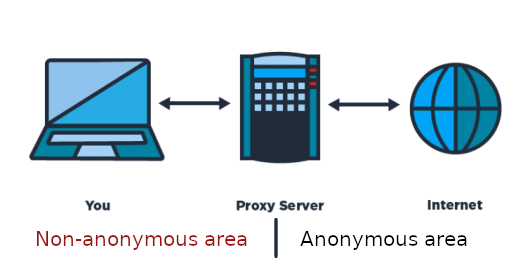
\includegraphics[width=.7\textwidth]{images/proxy2}
\end{figure}

Una \emph{proxy chain} (o cascata di proxy) prevede il passaggio del pacchetto da diversi server proxy nel tragitto dall'utente al destinatario. Ogni proxy conosce solo l'hop precedente ed il successivo, perciò basta un solo proxy non compromesso per evitare la compromissione dell'anonymity.
\begin{figure}[htp]
	\centering
	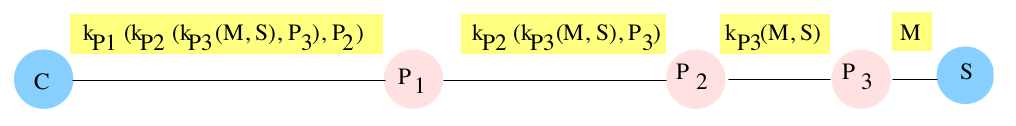
\includegraphics[width=\textwidth]{images/proxychain}
	\caption{Esempio di proxy chain.}
\end{figure}

Le cascate di proxy permettono di rendere anonimo il mittente, tuttavia il destinatario rimane visibile ed l'analisi del traffico è ancora possibile, per risolvere tali problemi introduciamo le mix networks.

\section{Mix networks}
L'anonimità del destinatario può essere garantita mediante l'invio di pacchetti in broadcast o multicast, tuttavia è raramente possibile usare tali metodi. Per questo furono sviluppate le \emph{mix networks}, pensate come meccanismo per stabilire canali anonimi.

Queste furono studiate per lavorare in un ambiente con attaccante di rete, il quale può:
\begin{itemize}
	\item capire origine e destinazione dei messaggi;
	\item inserire, rimuovere o modificare messaggi;
	\item \textbf{non} può mettere in relazione messaggi in chiaro e messaggi cifrati.
\end{itemize}
Un server \emph{Mix} è una variante del singolo proxy, con aggiunta di padding e cifratura.
\begin{equation*}
	\langle R_1, \langle R_0,M\rangle_{K_B},B\rangle_{K_1} \rightarrow \langle\langle R_0,M\rangle_{K_B},B\rangle
\end{equation*}
con $R_i$ sequenze casuali di bit.\\
Un server mix esegue ulteriori operazioni per impedire l'analisi del traffico.
\begin{enumerate}
	\item Oggetti di misura fissa (usando split o padding).
	\item Ordine di arrivo dei messaggi nascosto.
	\item Blocco dei messaggi ripetuti.
	\item Richiede un sufficente traffico di rete per funzionare.
\end{enumerate}
Un mix può anche ritornare una ricevuta $Y$ per i messaggi ricevuti:
\begin{equation*}
	Y = \langle C \langle R_1 \langle R_0, M\rangle_{K_B}, B \rangle_{K_1} \rangle_{K_1^{-1}}
\end{equation*}
con $C$ lunga sequenza costante di bit conosciuta, esempio: sequenza di zeri.
Un partecipante può in seguito dimostrare l'invio di un messaggio, garantendo la non-repudiation:
\begin{equation*}
	X = \langle\langle R_0, M\rangle_{K_B}, B \rangle \qquad \langle Y\rangle_{K_1} = \langle C \langle R_1, X \rangle_{K_1} \rangle
\end{equation*}
L'utilizzo di un singolo mix ha gli stessi problemi dell'utilizzo di un proxy, perciò riduciamo il rischi di compromissione creando una mix network. Se A deve mandare un messaggio a B, sceglie il percorso di mix server da seguire e cifra il messaggio di conseguenza. I mix del percorso scelto agiranno dunque come nel caso della proxy chain.

\noindent
Fasi del funzionamento di un mix:
\begin{enumerate}
	\item Scarta i messaggi ripetuti.
	\item Scarta i messaggi dummies ricevuti.
	\item Genera dei nuovi dummies.
	\item Invia a più destinazioni tutti i messaggi.
\end{enumerate}

Il destinatario tuttavia non conosce l'indirizzo del mittente, quindi non può rispondere. Per ovviare al problema, il mittente include nel messaggio l'indirizzo a cui rispondere. Esempio con singolo mix (chiave $K_1$):
\begin{colbox}{beige}{8cm}
	\begin{enumerate}
		\item $\fromto{A}{Mix}\{ R_1, \{R_0, M\}_{K_B}, B\}_{K_{mix}}$
		\item $\fromto{Mix}{B}\{\{R_0, M\}_{K_B}, B\}$
		\item $\fromto{B}{Mix}\{K_1, A\}_{K_{mix}}, \{R_2, M'\}_{K_2}$
		\item $\fromto{Mix}{A}A,\{\{R_2, M'\}_{K_2}\}_{K_1}$
	\end{enumerate}
\end{colbox}
dove $M$ contiene $\{\{K_1, A\}_{K_{mix}}, K_2\}$.

\begin{figure}[htp]
	\centering
	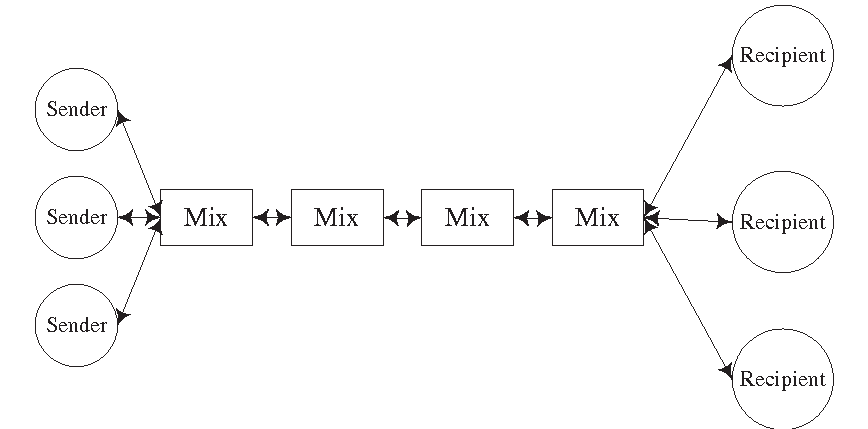
\includegraphics[width=\textwidth]{images/MixNetwork}
	\caption{Schema generico di una mix network.}
\end{figure}

\section{Anonymous networks}
Abbiamo introdotto il concetto di anonimato come lo stato in cui le proprie azioni sono indistinguibili da quelle di altri agenti appartenenti al medesimo anonymity set. Rendiamo più stringente questo concetto definendo la \emph{non osservabilità}: un osservatore non può affermare se una determinata attività abbia avuto luogo o meno.\\
Possibili attacchi all'anonimato:
\begin{itemize}
	\item \emph{Analisi passiva} del traffico.
	\item \emph{Analisi attiva} del traffico, con iniezione di pacchetti o firme temporali.
	\item \emph{Compromissione dei nodi} della rete (ipotesi: solo una parte è infetta).
\end{itemize}
Come abbiamo visto questi problemi sono risolvibili attraverso le mix networks, le quali tuttavia sono computazionalmente onerose a causa della cifratura a chiave pubblica, perciò risultano adatte allo scambio di mail ma non per altri scopi (esempio: web browsing).

Idee: randomizzare il routing e usare chiavi di sessione. Cambiare più volte il path dei messaggi rende più difficile effettuare un attacco, e usando una chiave di sessione possiamo rendere prestazionalmente accettabile l'uso di una mix network.

\subsection{Onion routing}
Per applicare le idee introdotte sopra, sfruttiamo un \emph{onion routing}, in cui il mittente decide il path e genera i layer di cifratura (a ``cipolla"), ipotizzando che alcuni nodi siano compromessi.
Il sistema più noto basato su onion routing di seconda generazione è \textbf{Tor}, che conta centinaia di nodi sparsi nel globo e può essere usato senza privilegi di amministratore per allargarne la base d'utilizzo.

L'architettura di Tor è pensata per mantenere segreti i server, per farlo vengono assegnati ad alcuni nodi i ruoli di \emph{introduction point} ed \emph{exit point}. Un utente che intende accedere ad un server della rete di Tor comunica con un intro point, scambiandosi una chiave di sessione. A questo punto contatta iterativamente un nuovo nodo, scambiandosi nuove chiavi, al fine di generare un path fino ad un exit point. Quest'ultimo nodo sarà incaricato di contattare il server per conto dell'utente e stabilire un punto di \emph{rendevouz}, al fine di non esporre il server.



\chapter{Intruders}
Un problema importante per i sistemi di rete riguarda il rischio di accessi ostili o non autorizzati, sia via rete sia localmente. Possiamo classificare gli intrusi come segue:
\begin{itemize}
	\item \emph{Masquerader}\\
	Utente non autorizzato ad accedere al sistema (outsider).
	\item \emph{Misfeasor}\\
	Utente legittimo che accede a dati o programmi a cui non avrebbe accesso o fa un uso improprio dei suoi privilegi (insider).
	\item \emph{Clandestine}\\
	Utente che prende il controllo del sistema e lo usa per impedire di essere rilevato o tracciato.
\end{itemize}
Un intruder punta ad ottenere l'accesso al sistema e, successivamente, a scalarne i privilegi, spesso sfruttando vulnerabilità. \`E inoltre importante riuscire a coprire le tracce.

Per poter ottenere i privilegi da amministratore è necessario impossessarsi della password. Indovinare la password è spesso la tecnica più efficace, ma se è troppo complicata risulta necessario catturarla mediante keylogger, trojan per ingannare l'utente o monitorando login su reti non sicure.

\section{Intrusion Detection}
Implementare un sistema privo di vulnerabilità è praticamente impossibile, perciò oltre a cercare di prevenire accessi indesiderati, dobbiamo sviluppare degli \emph{Intrusion Detection Systems} (IDS). Quest'ultimi hanno un duplice scopo: rilevare velocemente eventuali intrusioni e raccogliere informazioni per incrementare la sicurezza del sistema.

\begin{figure}[htp]
	\centering
	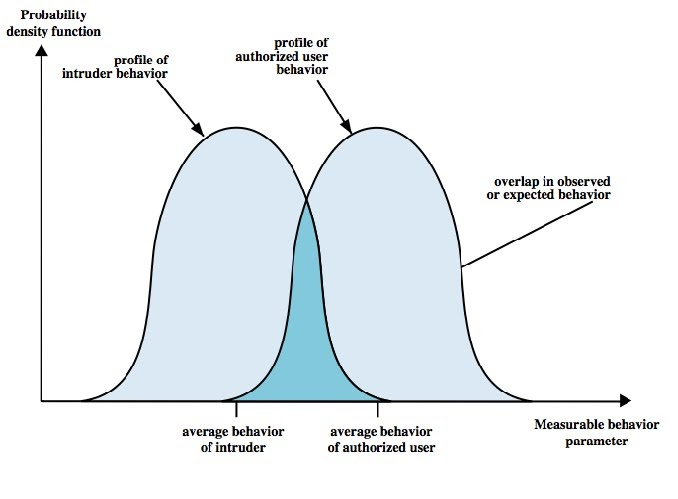
\includegraphics[width=.8\textwidth]{images/IDSprinciples}
\end{figure}

\noindent
Ci sono due approcci principali all'intrusion detection:
\begin{itemize}
	\item \emph{Statistical anomaly detection}
	\item \emph{Rule-based detection}
\end{itemize}
Inoltre gli IDS sfruttano file di \emph{audit}, in cui viene scritto ogni evento avvenuto nel sistema e l'autore di tale azione. Questi record sono nativi, quindi già predisposti all'uso in ogni sistema operativo multi-utente. Possono essere usati inoltre audit detection-specific che collezionano informazioni più specifiche, aggiungendo tuttavia overhead al sistema.


\subsection{Statistical anomaly detection}
Questo approccio si basa sulla definizione di \emph{comportamento normale} di un utente, puntando a riconoscere comportamenti illegittimi qualora determinati eventi si verificassero in modo inusuale.
Per fare ciò utilizza due meccanismi:
\begin{itemize}
	\item \emph{Threshold detection}\\
	Definisce delle soglie riguardanti le occorrenze di vari eventi, sospettando un'intrusione se il numero di eventi accaduti risulta eccessivo; inoltre le soglie sono indipendenti dall'utente. Se usato singolarmente è un meccanismo inefficace.
	\item \emph{Profile based}\\
	Per ogni utente cerca di sviluppare un profilo comportamentale e rileva evidenti variazioni dal comportamento atteso.
\end{itemize}

\subsection{Rule-based detection}
Questo secondo approccio punta a definire un \emph{comportamento legittimo}, osservando gli eventi che accadono nel sistema e applicando delle regole per capire se c'è rischio di intrusione. Le regole sono costruite in due modi:
\begin{itemize}
	\item \emph{Rule-based anomaly detection}\\
	Analizza lo storico degli audit per rilevare pattern comportamentali e generare automaticamente regole ad-hoc, verificando che l'attuale comportamento sia conforme ad esse.
	\item \emph{Rule-based penetration identification}\\
	Le regole vengono inserite manualmente da esperti in base ad attacchi noti e vulnerabilità del sistema per rilevare attacchi specifici.
\end{itemize}

\noindent
NB: Un buon IDS non solo deve rilevare rapidamente più intrusioni possibili, ma deve anche generare pochi falsi positivi! 

\subsection{Distributed Intrusion Detection}
Gli IDS tradizionali si concentrano su un singolo sistema, ma spesso siamo costretti a proteggere sistemi distribuiti, per esempio una rete locale. Dobbiamo perciò gestire nuove tematiche, tra cui la gestione degli audit (formato, consistenza), l'integrità e la confidenzialità dei dati, la scelta di un'architettura centralizzata o distribuita per il rilevamento di intrusioni. L'architettura più comune è così articolata:
\begin{itemize}
	\item \emph{Host agent}: moduli dei singoli PC che raccolgono audit.
	\item \emph{LAN agent}: analizzano il traffico di rete.
	\item \emph{Central manager}: analizza report o direttamente gli audit per trovare eventuali anomalie o segni di intrusione.
\end{itemize}

\begin{figure}[htp]
	\centering
	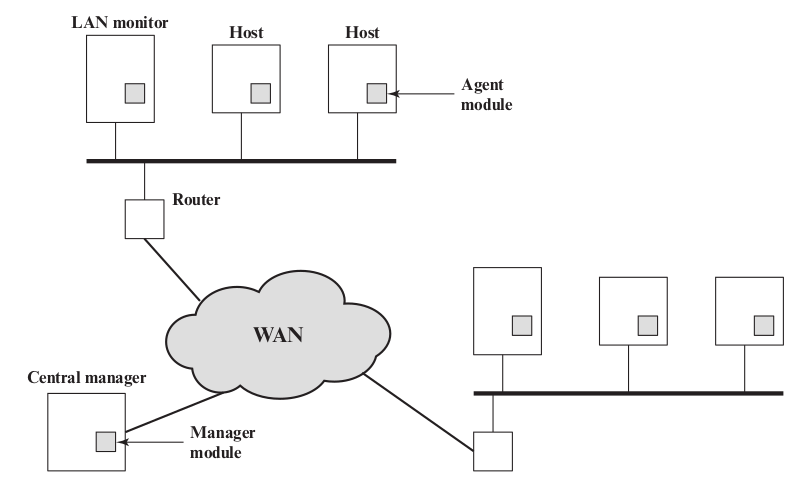
\includegraphics[width=.9\textwidth]{images/LANIDS}
	\caption{IDS per sistemi distribuiti.}
\end{figure}

\subsection{Honeypot}
Sistemi che fungono da esca per l'attaccante. Essi devono sembrare dei veri e propri sistemi, ben difesi e con file apparentemente importanti all'interno. Sono isolati rispetto ai dati sensibili del vero sistema e sono usati per studiare le attività di un attaccante.


\chapter{Firewall}
Un \emph{firewall} è un \emph{Intrusion Prevention System} (IPS) e funge da punto di controllo e monitoraggio del traffico di rete. Esso interconnette reti con differenti livelli di fiducia, impone restrizioni ai servizi di rete e permette auditing e controllo degli accessi.
Un firewall dev'essere immune ad attacchi esterni, tuttavia non può proteggere da:
\begin{itemize}
	\item Attacchi che bypassano il controllo (esempio: servizi trusted).
	\item Minacce interne.
	\item Attacchi attraverso la rete locale.
	\item Malware eseguiti all'interno del sistema.
\end{itemize}
Possiamo trovare firewall di varie tipologie in base a dove si collocano nella pila ISO/OSI.

\section{Tipologie di firewall}
\subsection{Packet Filters}
Tipologia di firewall più semplice e veloce. Questi si basano sull'analisi dei campi dei pacchetti IP senza tener traccia del contesto, accettandoli o scartandoli in base a regole specifiche.
Sono usualmente collocati sulle interfacce di ingresso e uscita del gateway.\\
Prevedono politiche predefinite:
\begin{itemize}
	\item Ciò che non è espressamente consentito è proibito (default deny).
	\item Ciò che non è espressamente proibito è consentito (default allow).
\end{itemize}
Un possibile attacco è detto \emph{IP address spoofing}, in cui l'attaccante invia pacchetti dall'esterno, impostando come IP di origine uno di quelli della rete interna al firewall. Questo attacco non funziona più in quanto i firewall distinguono interfacce interne ed esterne.

\subsection{Stateful Packet Filters}
A differenza del tipo precedente, questi firewall memorizzano un contesto per poter applicare regole più complesse al traffico di rete. Essi tengono traccia delle sessioni in corso o in fase di apertura per accettare tutti e soli i pacchetti validi.

\subsection{Application Level Gateway/Proxy}
Firewall specifici per applicazioni, eseguiti su gateway o proxy, che possono controllare se l'utente è autorizzato a fare una determinata richiesta. Ogni applicazione necessita di un proxy specifico, invece di un unico proxy per gestire più servizi, in questo modo il sistema risulta più robusto a eventuali falle e non ha un unico punto di rottura.

\subsection{Circuit Level Gateway}
Firewall a livello di trasporto che permettono di impostare dei ``circuiti sicuri", il cui traffico non viene analizzato, basandosi sulla fiducia negli utenti interni.

\section{Posizionamento del firewall}
\subsection{Bastion Host}
Host reso particolarmente sicuro, incaricato di eseguire firewall a livello applicativo o di trasporto e di fornire accesso ai servizi esterni. Essendo esposto a possibili minacce presenta un sistema operativo più robusto, solo i servizi essenziali e richiede autorizzazioni aggiuntive.

\subsection{Host-based firewall}
Firewall sviluppati per essere eseguiti su host individuali, ad esempio su un server. Questi sono disponibili nativamente in molti sistemi operativi e permettono di configurare regole di filtraggio in base all'ambiente in cui sono collocati.

\subsection{Personal firewall}
Questa tipologia di firewall è solitamente meno complessa ed è pensare per essere eseguita sul proprio PC o sul router di casa. Il suo scopo principale è bloccare accessi remoti non autorizzati a computer o risorse della rete locale e impedire il monitoraggio di eventuali malware.


\section{DMZ e VPN}
Mostriamo attraverso le seguenti immagini come vengono usati i firewall per instaurare e rendere garantire la sicurezza di \emph{zone demilitarizzate} (DMZ) e \emph{reti virtuali private} (VPN).
\begin{figure}
	\centering
	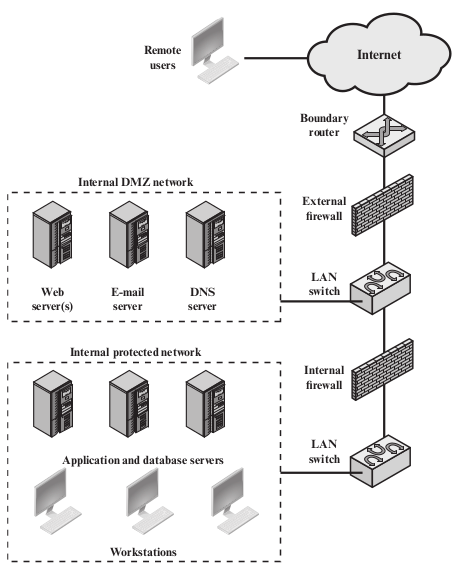
\includegraphics[width=.7\textwidth]{images/firewallSchema}
	\caption{Disposizione dei firewall per stabilire una DMZ.}
\end{figure}
\begin{figure}
	\centering
	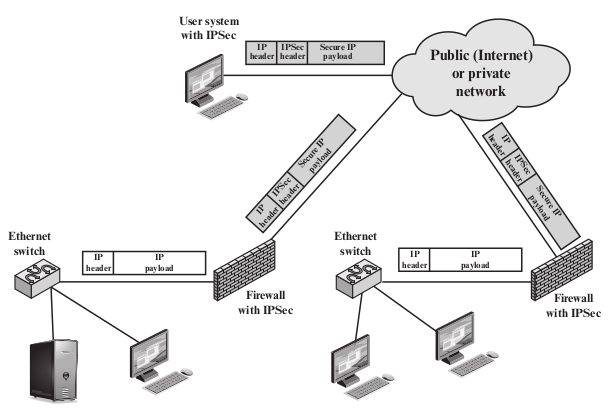
\includegraphics[width=.9\textwidth]{images/VPN}
	\caption{Utilizzo dei firewall in una VPN.}
\end{figure}




\end{document}